\chapter{\label{ch-experimentAnalysis} Measuring the TMPTA principal Hugoniot: analysis and interpretation}

\minitoc

\section{Introduction}

This chapter will outline the steps taken to analyse the data from Chapter \ref{ch-experiment}. The results will then be discussed and compared with simulation and previous experimental results, and some unexpected features in the data investigated. 

In Section \ref{VISAR analysis}, the analysis of the VISAR data will be discussed, showing how the streak images can be used to calculate the shock state achieved in the foam on each shot. Section \ref{SOP analysis} focuses on the SOP data, describing how this was used to calculate the shock temperature, and how SOP timing data could be compared to that obtained from the VISAR. Section \ref{Other diagnostic analysis} then looks at the information that could be obtained using the fiducial, pinhole camera, and photodiode traces of the laser pulse. The data analysis then concludes with Section \ref{Data choices}, which broadly describes how decisions were made regarding the final data set.

The main results are then discussed in Section \ref{Experiment Results}, where they are compared to both theoretical models and data from previous experiments on similar materials. Comparison with post-experiment simulations is then presented in Section \ref{Post shock simulations}. Section \ref{Weak quartz shock} then describes how a certain feature of the data - a weaker than expected shock in the quartz - was investigated, and explores a potential explanation for this. Finally, Section \ref{Suggested Improvements} discusses suggested improvements that could be made were such an experiment to be performed again.

The structure used here has been chosen to aid explanation of the results, and roughly follows how it was actually performed. However, the analysis was in reality an iterative process; early stages were refined and revised later on, and early results from the preliminary analysis meant that this was performed with some knowledge of the final data set. A basic confidence ranking had to be performed early on to obtain preliminary results and spot trends in the data, and this was then updated as understanding and interpretation of the data set improved. In recognition of this, the results from each stage of the described analysis will be included in that section, although these will not be discussed in detail until Section \ref{Experiment Results}. The data set used in these results is the data set selected in Section \ref{Data choices} (highlighting the iterative nature of this analysis).

Throughout this chapter, experimental data is displayed to aid understanding of the analysis. For consistency, wherever possible data from the same shot has been used, but this was not always possible. Shot 38 is used for the general VISAR and SOP analysis, as this shot contained the clearest data. However, it did not have a fiducial present, which meant that the ablator/gold transit times could not be determined - the simulations therefore focus instead on an alternative shot, Shot 47. Data from other shots are also sometimes used where necessary to best show a particular feature or behaviour.

%I performed the work described in this chapter, and wrote the code in which the analysis was performed. I also performed a large amount of the simulation work, and interpreted the data. I have included some work performed by the other experimental collaborators, and have indicated where this arose. This was predominantly in the analysis of the curved VISAR data (where I performed the analysis based on code written by Daniel Eakins), and in the simulation work, where Multi and some of the Helios simulations were performed by Paul Neumayer and Artem Martynenko, and the Flash simulations were performed by Piotr R\k{a}czka.

\section{Analysis of VISAR data} \label{VISAR analysis}
%\subsection{Collected data for a typical shot}

%The data collected for a typical shot is consisted of:
%\begin{itemize}
%\item Photos of the target (taken by target fabrication)
%\item Measurements of the target dimensions (performed by target fabrication)
%\item Measurements of the energy of each beam (from the on-shot calorimetry)
%\item Traces of the pulse profile of the beams (taken from photodiodes viewing parasitic signal from a lossy-mirror)
%\item Images from each VISAR streak camera (one from each, two in total)
%\item Image from the SOP streak camera (one - containing fiducial signal from start of beam)
%\end{itemize}

\subsection{Identifying shock velocities from raw VISAR data}

In the VISAR streak images, the x-axis position is a spatial dimension, and the image contains two distinct halves - one corresponding to the quartz, and the other to the foam. The y-direction represents time, with later times at the bottom of the image. A labelled example can be seen in Figure \ref{fig:VISARImage}. Three `transitions' can be identified in the image. Firstly, shock entry into the quartz can be identified by a sudden change in signal intensity on the quartz half of the image. Secondly, shock breakout from the quartz rear-surface can be identified by fringe extinction on this half. This also corresponds to the shock entering the foam (although as the foam is opaque to the probe laser, no change is seen in the foam signal at this point). Finally, shock breakout in the foam could be identified by fringe extinction on the foam half of the image.

\begin{figure} [h]
\begin{centering}
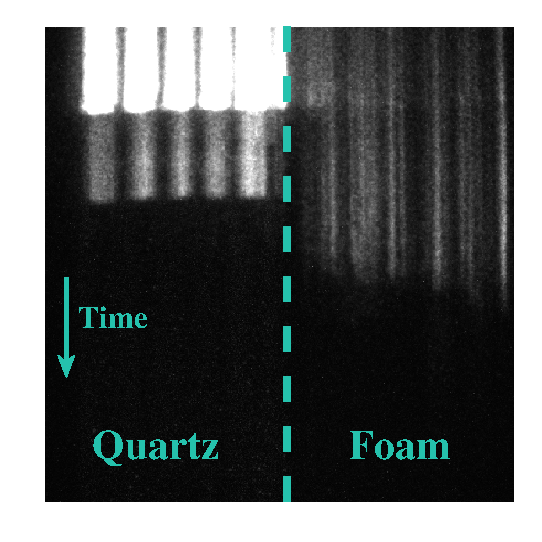
\includegraphics[width=0.5\textwidth]{figures/Experiment/VISARImage.eps}% Here is how to import EPS art
\caption{\label{fig:VISARImage} A raw VISAR streak image for shot 38, labelled to indicate the quartz and foam signals. Three clear changes can be observed; a change in fringe intensity in the quartz (corresponding to the shock entering the quartz from the gold), fringe extinction in the quartz (shock breakout from the quartz), and fringe extinction in the foam (shock breakout from the foam). }
\end{centering}
\end{figure}

The two VISAR images for each shot were considered together. In each image, where possible, the time at which these three changes in behaviour occurred were identified. These changes typically occurred over a range of pixels (rather than at a single clear point), and so a `region of interest' was selected for each to cover the full range over which the transition could possibly have occurred. Example selections are displayed in Figure \ref{fig:VISAR ROI}.

\begin{figure} [h]
\begin{centering}
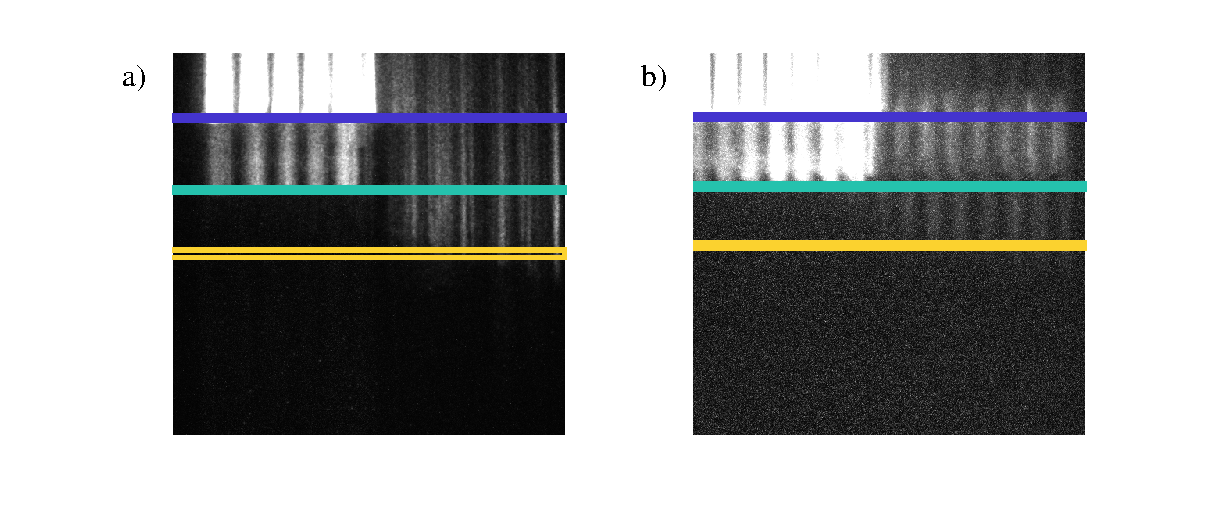
\includegraphics[width=1.0\textwidth]{figures/Experiment/VISARROI.eps}% Here is how to import EPS art
\caption{\label{fig:VISAR ROI} VISAR images from the two VISARs for shot 38. The selected regions where the shock transitions are believed to be confirmed are shown. The blue region corresponds to shock entry into the quartz, while the teal region corresponds to shock breakout from the quartz and the yellow corresponds to shock breakout from the foam. The edge of image (a) appears to show some curvature; this is expected based on the simulations due to the size of the VULCAN laser spot. The region was chosen to capture the transition at the centre, where the shock is expected to be more planar.}
\end{centering}
\end{figure}

The streak time was then used to convert the pixels (in the y-direction) to time. The ROI's were thus converted from a pixel range into a time (the mean position of the window) with associated uncertainty (the width of the window). The finite slit width of the camera also introduced a minimum possible time resolution (which was used for the uncertainty if the ROI width was less than this value). The differences between these three timings were then used to calculate the shock transit time through the quartz and the foam.

For many shots, the timings could only be confidently determined from a single VISAR. In these cases, only the transit times from that image were used for the analysis. When both VISARs returned good data, these two independent measurements could be used to reduce the uncertainty; a single transit time (with smaller uncertainty) could be produced, corresponding to the range of values compatible with both diagnostics. 

Finally, the thickness of the quartz and foam layers (with estimated uncertainties) were then used to calculate the average shock velocity in each material. The shock velocity calculated for a single shot using the independent time measurements from each VISAR, along with that calculated from the combined time measurements, are shown in Figure \ref{fig:VISAR Timing}.

\begin{figure} [h]
\begin{centering}
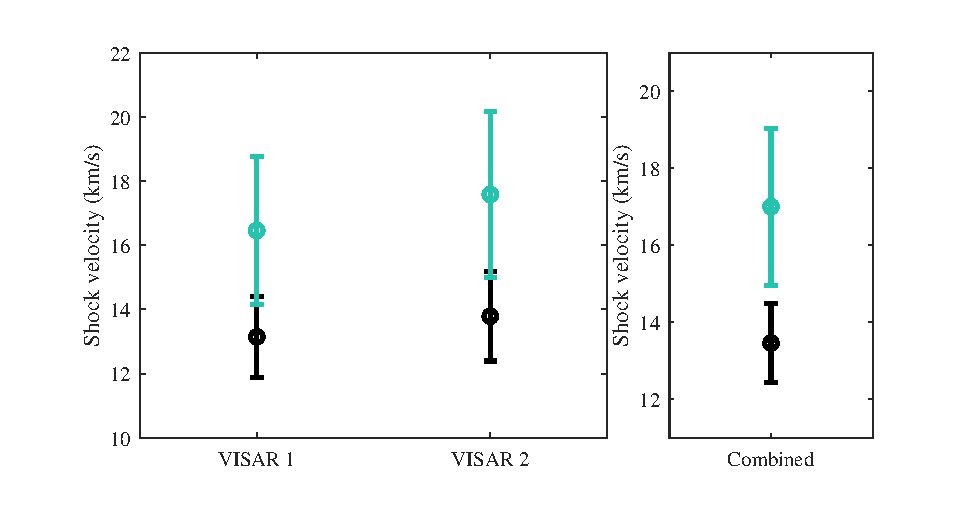
\includegraphics[width=1.0\textwidth]{figures/Experiment/VISARTiming.eps}% Here is how to import EPS art
\caption{\label{fig:VISAR Timing} Calculated shock velocities in the quartz (black) and the foam (teal)  for shot 38, using the shock timings obtained from the VISAR images in Figure \ref{fig:VISAR ROI}. In this shot, all three timings can be identified from both VISARs. The shock velocities corresponding to the timing data from each of the two VISARs independently is displayed, along with the shock velocity calculated from the `combined' timings. The combined measurement uses both sets of VISAR measurements to reduce the error, giving a `combined' set of possible timings that is compatible with the uncertainty ranges measured by each VISAR.}
\end{centering}
\end{figure}

%An attempt was made at this point to identify the same three transitions from the SOP data, to provide another measure of these shock transit times. However, this turned out not to be possible - there was no clear change in the SOP data correlating to the shock breakout from the quartz, which prevented either shock breakout time from being calculated. It was also found that the start of the foam self-emission occurred before the shock breakout in the VISAR images (likely indicating some transparency of the foam to these self-emitted frequencies).


\subsection{Impedance matching calculation} \label{IM calc}
The impedance matching calculation was then performed to calculate the foam shock state from the two shock velocity measurements. The principles behind this calculation is described in Sections \ref{IMTheory} and \ref{IMTheoryMeasurements}, where case the quartz is the reference material (for which the Hugoniot and release isentrope are known) and the foam is the material of study.

An initial faster but less accurate impedance matching calculation was performed to assess the data (and to provide a sanity check on the more accurate, but more complicated, subsequent calculation). This used a common assumption that the quartz release isentrope can be approximated by reflecting the quartz hugoniot around the quartz shock state. This is a reasonably accurate approximation at low pressures, but can introduce errors as the pressure is increased \cite{Forbes2012}. In this calculation, the quartz Hugoniot described in \cite{Knudson2009} was used, with a functional form of 
\begin{equation} \label{eqn:Old Hugoniot} U_s = a + b u_p - c u_p \exp{-d u_p}, \end{equation}
with coefficients of $a = 6.26 \pm 0.35$ \unit{\kilo\meter\per\second}, $b = -1.20 \mp 0.02$ , $c = 2.56 \mp 0.15$, and $d = 0.37 \pm 0.02$ $(\unit{\kilo\meter\per\second})^{-1}$. Then, as described in Section \ref{IMTheoryMeasurements}, the measured shock velocities were used to produce the quartz and foam Rayleigh lines. The intercept of the quartz Rayleigh line with quartz Hugoniot was used to determine the quartz shock state. The quartz Hugoniot was then reflected about this state, and the intercept of this approximate release isentrope with the foam Rayleigh line allowed the foam shock state to be calculated. This calculation was performed for each shot, and the preliminary results indicated that there was indeed a trend in the data and thus that the more complicated analysis should be conducted.

%A common approximation in impedance matching calculations is not to calculate the release isentrope, but instead to reflect the hugoniot of the reference material (for this experiment, quartz) around the reference material (quartz) shock state. For low pressures this is reasonably accurate, but it can introduce errors as the pressure is increased. An initial calculation was performed using this approach to produce a first estimate of the results, and to provide a sanity check on the results of the more complicated (but more complete) approach. In this calculation, the Hugoniot described in \cite{Knudson2009} was used: \begin{equation} \label{eqn:Hugoniot} U_s = \sum_{n=0}^3 a_n u_p^n \;, \end{equation} with coefficients in Table \ref{tab:HugoniotCoeffs} \cite{Knudson2013} - a cubic fit to experimental data from \cite{Knudson2009} The intercept of this Hugoniot with the quartz Rayleigh line,  $P = \rho_0^{quartz} U_s^{quartz} u_p$, where $P$ is Pressure, $u_p$ is particle velocity, and $U_s^{quartz}$ is the measured quartz shock velocity, was found. This intercept provided ($P^{quartz}, u_p^{quartz}$), the quartz shock state. The Hugoniot was then reflected around this point to approximate the release isentrope. The intercept of this reflected Hugoniot with the foam Rayleigh line, $P = \rho_0^{foam} U_s^{foam} u_p$, was then found, which defined the foam shock state ($P^{foam}, u_p^{foam}$). This was performed for each shot.

\begin{table}%The best place to locate the table environment is directly after its first reference in text
\centering
\caption{\label{tab:HugoniotCoeffs}%
Coefficients for the quartz Hugoniot in equation \ref{eqn:Hugoniot}, reproduced from \cite{Knudson2013}.
}
\begin{tabular}{lccr}
\hline\hline
\textrm{$a_0$ \si[per-mode=symbol]{(km/s)}}&
\textrm{$a_1$}&
\textrm{$a_2$ \si[per-mode=symbol]{\kilo\meter\per\second} }&
\textrm{$a_3$ \si[per-mode=symbol]{(km/s)^{-2}} } \\
\hline
1.754 & \num{1.862} & \num{-3.364E-2} & \num{5.666E-4}\\
\hline\hline
\end{tabular}
\end{table}

The more accurate calculation used a full and complete calculation of the release isentrope. For this version of the impedance matching calculation a slightly different functional form for the Hugoniot was used \cite{Knudson2013} - a cubic fit to the same data as used previously \cite{Knudson2009}. The new Hugoniot was described by \begin{equation} \label{eqn:Hugoniot} U_s = \sum_{n=0}^3 a_n u_p^n \;, \end{equation} with coefficients in Table \ref{tab:HugoniotCoeffs}. This newer form was used to facilitate the use of Monte Carlo error analysis (described in Section \ref{MC error}). The release isentrope was then accurately calculated according to the relevant quartz shock state. This was done largely according to the method outlined by Knudson and Desjarlais \cite{Knudson2013}, but with a few small differences. 

In their paper, Knudson and Desjarlais model the isentrope using a new `linear-reference' Mie-Gruneison model. The key departure of this model from other approaches is the use of a variable Gr{\"u}neisen parameter. They compare the new model to the previous standard - a conventional Mie-Gruneison model with a fixed Gr{\"u}neisen parameter of $\Gamma = 0.64$ - and found that the new model led to reduced errors. However, the range of pressures over which this model is valid does not extend across those achieved in this experiment, and the model  returned implausible results for some of these values. As such, the conventional Mie-Gruneison model, with a fixed Gr{\"u}neisen parameter of $\Gamma = 0.64$, was used. This value of the Gr{\"u}neisen parameter was calculated from a range of EOS models \cite{Hicks2008}, and is in good agreement with that derived \cite{Hicks2008} from experiments \cite{Hicks2005, Trunin1994}. Other than this change to the Gruneison parameter, the method for calculating the release isentrope for a given quartz shock state was as Knudson and Desjarlais described \cite{Knudson2013}.

The impedance matching calculation was therefore conducted as in the previous method, with this more accurate model for the quartz isentrope used, and the foam shock ($u_p^{foam}, P^{foam}$) state was determined from the intercept of this curve with the foam Rayleigh line. A graphical representation of this for the experimental data from Shot 38 is shown in Figure \ref{fig:Impedance Match}. This calculation was performed for all shots. A comparison with the previous method, using the reflected Hugoniot as the isentrope, found the difference to be essentially negligible; this suggests the isentrope is comparable to the reflected Hugoniot in this regime, and provided a sanity check that the release isentrope had been calculated correctly.

%The calculation follows that described for the reflected-Hugoniot model, except that once the quartz shock state ($P^{quartz}, u_p^{quartz}$) has been found, the associated isentrope for that state is calculated following the method described in appendix. This is then used in place of the reflected Hugoniot. Once this had been performed for all shots, the results of this calculation were compared to the reflected hugoniot ones, and the difference was found to be negligible. A graphical representation of this imedance matching calculation is shown in Figure \ref{fig:Impedance Match}.

\begin{figure} [h]
\begin{centering}
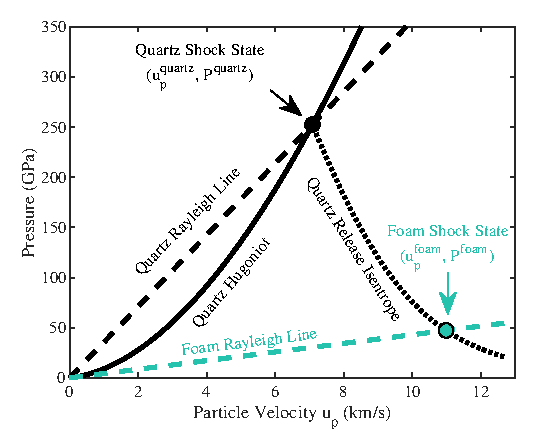
\includegraphics[width=0.6\textwidth]{figures/Experiment/ImpedanceMatch.eps}% Here is how to import EPS art
\caption{\label{fig:Impedance Match} The impedance matching calculation for the shock velocities obtained from shot 38. The intercept of the quartz Rayleigh line and the quartz Hugoniot defines the quartz shock state. The release isentrope for this shock state is then calculated, and the intercept of this curve with the foam Rayleigh line describes the foam shock state.}
\end{centering}
\end{figure}

The resulting foam shock states for the final data set are displayed in Figure \ref{fig:Hugoniot}, where they are compared to theoretical models. These results will be discussed in Section \ref{Experiment Results}. The error bars are calculated as explained in Section \ref{MC error}.

\begin{figure} [h]
\begin{centering}
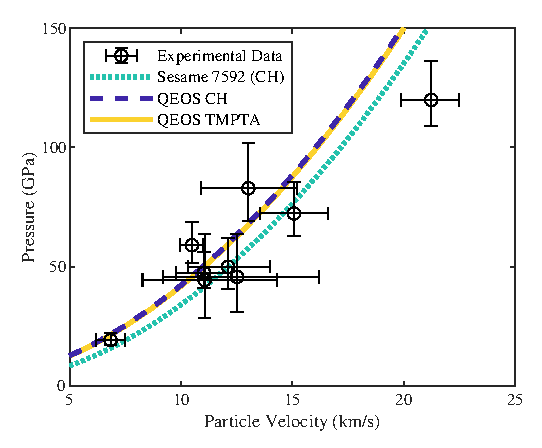
\includegraphics[width=0.6\textwidth]{figures/Experiment/Hugoniot.eps}% Here is how to import EPS art
\caption{\label{fig:Hugoniot} The foam hugoniot data calculated from the impedance matching calculation, compared to hugoniots generated from theoretical equation of state models.}
\end{centering}
\end{figure}


\subsection{Uncertainty quantification - Monte Carlo analysis} \label{MC error}

Uncertainty quantification for the shock variables obtained using the impedance matching calculation was performed using a Monte Carlo approach \cite{Root2010}. This technique allowed the experimental uncertainty to be propagated through the complex IM calculation, while also including uncertainty contributions from the quartz hugoniot fit and foam initial density. This section is accompanied by a flow chart in Figure \ref{fig:MC Flow Chart}, which shows the different steps of this calculation for shot 38 with example distributions and samples. Uncertainty quantification in this way has previously been performed on other similar experiments \cite{Knudson2013, Root2010, Root2013, McCoy2016}.

%My initial solution to this problem was to perform each calculation three times for a single shot. Consider the IM calculation as a black box, which takes inputs (shock velocities) and returns outputs (shock pressures, particle velocities etc.). If we take an input of $A \pm B$, the calculation was performed for A, A + B, and A - B. This would return answers of C, D, and E - where C is the 'value' we would then use, and D and E are the ranges of our uncertainties. This approach worked, but lacked elegance. It was difficult to include Hugoniot error, and it also required careful thought to ensure the right 'sets' of inputs were included to make sure the uncertainties summed in the right way. This approach also had statistical flaws - I was finding max errors by assuming that each input had it's maximal error at the same time (a worst-case scenario), but this is more pessimistic than standard error propogation formulas, and thus led to larger errors.

The calculation begins with the measured shock velocities for the quartz and foam for a particular shot. These are of form $U_{shock} \pm \epsilon$; a quoted value $U_{shock}$, with an experimentally measured error $\epsilon$ that is symmetric around this value. A normal distribution is then produced for each of the two shock velocities, with a mean of $U_{shock}$ and a standard deviation of $\epsilon$. 

These distributions were then used to perform 10,000 Monte Carlo iterations of the impedance matching calculation for each shot. For each iteration, a sample is randomly generated for each shock velocity and the foam density according to the relevant distribution. Samples are also generated for each of the four Hugoniot fit parameters, according to the covariance matrix\footnote{The printed matrix is that provided by \cite{Knudson2013}, but actually attempting to use this to generate the parameters returned an error due to the matrix not being positive definite. To resolve this, a small correction was added, $C + \num{1e-10}\cdot I$ was required, where $I$ is the identity matrix \cite{Holton2003}.} provided in \cite{Knudson2013},
\[C = 
\begin{bmatrix}
\num{2.097e-2} & \num{-6.159e-3} & \num{5.566e-4} & \num{-1.572 e-5}\\
\num{-6.159e-3} & \num{1.877e-3} & \num{-1.742e-4} & \num{5.017e-6}\\
\num{5.566e-4} & \num{-1.742e-4} & \num{1.650e-5} & \num{-4.834e-7}\\
\num{-1.572 e-5} & \num{5.017e-6} & \num{-4.834e-7} & \num{1.438e-8}\\
\end{bmatrix}. 	
\]

The impedance matching calculation was then performed, as described in Section \ref{IM calc}, using these randomly sampled values. The 10,000 iterations produced 10,000 different estimates of the quartz and foam shock states, providing distributions for each of the relevant shock variables. The standard deviations $\sigma$ of these distributions were then calculated, and used to define the uncertainty range of these values.


%\begin{table}%The best place to locate the table environment is directly after its first reference in text
%\caption{\label{tab:HugoniotCovariance}%
%Coefficients for the quartz Hugoniot in equation \ref{eqn:Hugoniot}, reproduced from \cite{Knudson2013}.
%}

%\begin{tabular}{lccccccccr}
%\hline\hline
%\begin{tabular}{@{}c@{}}$\sigma_{a_0}^2$ \\ $(\times 10^{-2})$\end{tabular}
%\begin{tabular}{@{}c@{}}$\sigma_{a_0}\sigma_{a_1}$ \\ $(\times 10^{-3})$\end{tabular}
%\begin{tabular}{@{}c@{}}$\sigma_{a_0}\sigma_{a_2}$ \\ $(\times 10^{-4})$\end{tabular}
%\begin{tabular}{@{}c@{}}$\sigma_{a_0}\sigma_{a_3}$ \\ $(\times 10^{-5})$\end{tabular}
%\begin{tabular}{@{}c@{}}$\sigma_{a_1}^2$ \\ $(\times 10^{-3})$\end{tabular}
%\begin{tabular}{@{}c@{}}$\sigma_{a_1}\sigma_{a_2}$ \\ $(\times 10^{-4})$\end{tabular}
%\begin{tabular}{@{}c@{}}$\sigma_{a_1}\sigma_{a_3}$ \\ $(\times 10^{-6})$\end{tabular}
%\begin{tabular}{@{}c@{}}$\sigma_{a_2}^2$ \\ $(\times 10^{-5})$\end{tabular}
%\begin{tabular}{@{}c@{}}$\sigma_{a_2}\sigma_{a_3}$ \\ $(\times 10^{-7})$\end{tabular}
%\begin{tabular}{@{}c@{}}$\sigma_{a_3}^2$ \\ $(\times 10^{-8})$\end{tabular} \\
%\hline
%2.097 & -6.159 & 5.566 & -1.572 & 1.877 & -1.742 & 5.017 & 1.650 & -4.834 & 1.438\\
%\hline\hline
%\end{tabular}
%\end{table}



The mean of the MC distribution of a particular value does not always equal the `exact' value obtained if the IM calculation is performed without considering uncertainty (i.e. if no MC sampling is performed, and thus for all shock velocities $U_{shock} \pm \epsilon$ the values of $U_{shock}$ are used, along with the exact Hugoniot fit parameters quoted in Table \ref{tab:HugoniotCoeffs}). This was most noticeable for the shock pressure, where there is a small amount of skew in the distribution\footnote{Skew in the MC distributions of such an experiment was also previously noted in \cite{Root2013}.} (the particle velocity distributions are effectively normal). This effect arises from a non-linearity in the calculation. Consider a shock velocity $U_{shock}$ and associated pressure $P$. A small positive increase in $U_{shock}$ results in a larger change in $P$ than a small decrease in $U_{shock}$, leading to a distribution mean that is skewed towards higher values.

The most obvious way to present the results of this calculation would be to quote each shock variable as the MC mean plus/minus the standard deviation. This could lead to confusion; for instance, the quartz shock state would then be quoted as $\bar{u_p}^{quartz} \pm \sigma_{u_p^{quartz}}$ and $\bar{P}^{quartz} \pm \sigma_{P_{quartz}}$ (where a variable with a bar is used to indicate the MC distribution mean), but the state ($\bar{u_p}^{quartz}, \bar{P}^{quartz}$) would not actually be a valid state on the quartz Hugoniot described by Equation \ref{eqn:Hugoniot}. To avoid this, the shock variables are instead quoted as the `exact' values - those obtained if the IM calculation is done without random sampling of any of the variables. These values are quoted with asymmetric error to describe the same uncertainty range as the standard deviation (which was symmetric about the mean). This is shown in the last box of Figure \ref{fig:MC Flow Chart}, where one standard deviation $\sigma$ from the mean (solid black line) is described by asymmetric errors $\epsilon_+$ and $\epsilon_-$ around the `exact' quoted value (orange) \footnote{It is also worth noting that the difference between the mean and the exact value is relatively small, and this uncertainty range actually represents 34\% (i.e. $1 \sigma$) of the generated MC samples in either direction from the `exact' value to within one or two percent).}.

%While the resulting distributions for the particle velocity were effectively normal, there was some noticeable skew in the Pressure distribution. This meant that the mean of the distribution was different to the value obtained for an `exact' impedance match calculation (note: in this case, `exact' is used to mean that for a shock velocity $U_{shock}$ with uncertainty $\epsilon$, quoted as $U_{shock} \pm \epsilon$, the calculation is performed for a value of $U_{shock}$ using the hugoniot parameters quoted in \label{tab:HugoniotCoeffs}). This difference is due to the non-linearity of the calculation; and indeed, an individual sample that used the `exact' shock velocities and Hugoniot parameters would return the exact outputs. Consider the exact pair $U_{shock}$ and $P$. If there is a small deviation $+ \delta$ from $U_{shock}$ in the positive direction, the resulting deviation from $P$ is larger than if there is a small deviation $- \delta$ in the negative direction. This shifts the mean to higher values. It is also worth noting that, as the number of MC samples tends towards infinity, the median of the MC samples tends towards the exact values. 

%Using the mean of the distributions would result in quoted values that were not consistent with the `exact' Hugoniot (i.e. the quoted ($P^{quartz}, U_s^{quartz}$) would not actually lie on the Hugoniot given by the quoted parameters in Table \ref{tab:HugoniotCoeffs}). To avoid this inconsistency, the `exact' value of each variable was used when quoting values - and so the values reported in the results section are those that would be achieved if the exact impedance matching calculation is performed on the quoted shock velocities. However, the calculated uncertainty - being the standard deviation of the distribution - is centered on the distribution mean, rather than this exact value. This means that the error bars that accompany the quoted values are asymmetric, as they are centered on the mean, rather than the `exact' value. These error bars still represent 34\% (i.e. $1 \sigma$) of the generated MC samples in either direction from the `exact' value to within one or two percent.

\begin{landscape}
\begin{figure} 
\begin{centering}
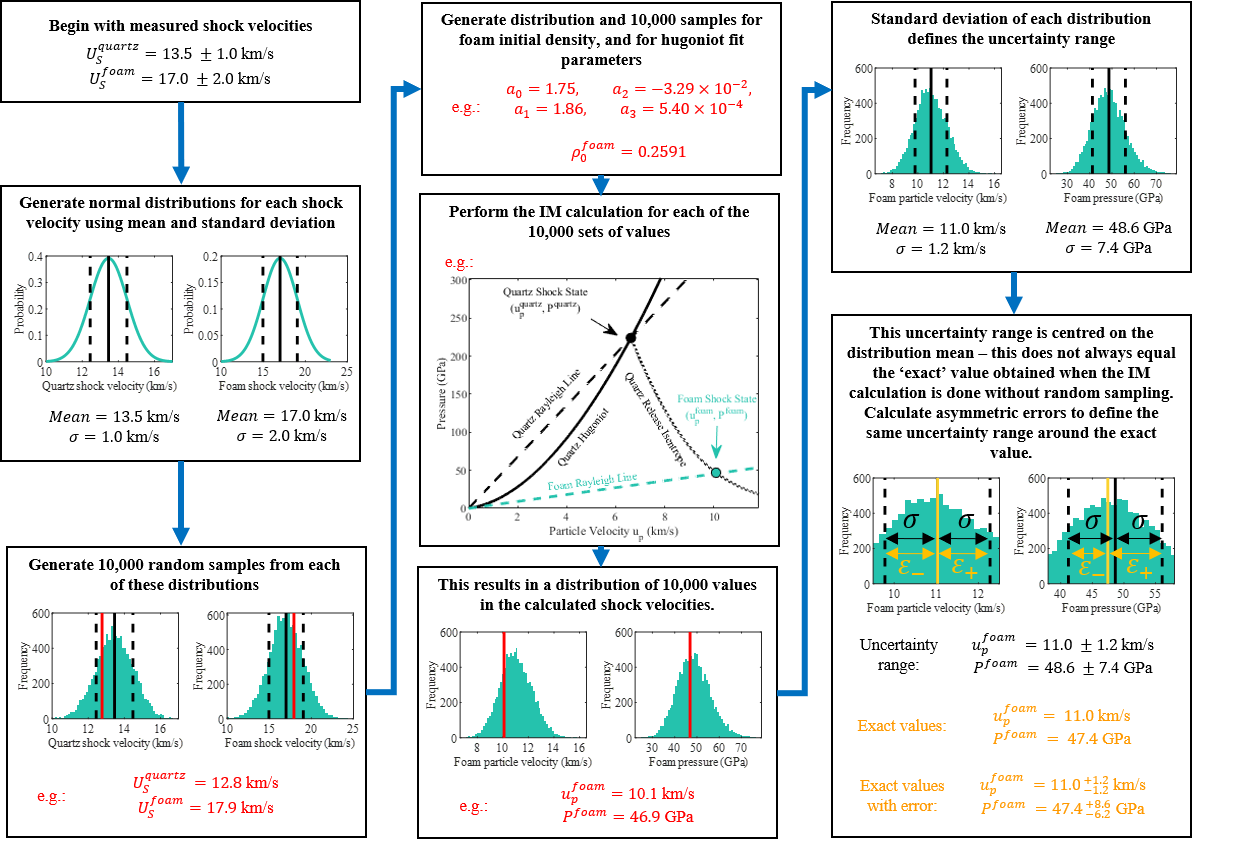
\includegraphics[width=1.5\textwidth]{figures/Experiment/FlowChart.png}% Here is how to import EPS art
\caption{\label{fig:MC Flow Chart} Flow chart showing the MC methodology for quantifying the uncertainty in the calculated variables. The MC analysis is shown for shot 38. The values/lines in red show the IM calculation performed for an example random sample from the set of the 10,000 random samples.}
\end{centering}
\end{figure}
\end{landscape}


\subsection{Achieved quartz shock states} \label{Achieved quartz shock states}

The achieved shock states in the quartz are displayed in Figure \ref{fig:QuartzShockStates}. This plot includes the eight shots from the main dataset, plus an additional two shots\footnote{These two shots were not included in the main dataset because of the lack of foam signal, but the quartz velocity could be calculated with confidence. In one, the target did not contain a foam layer. The other did have a foam layer, but the signal was too weak for foam breakout to be detected.}. As the quartz particle velocity and pressure were not measured directly, but were inferred using the hugoniot based on the measured shock velocity, these data points all lie perfectly on the hugoniot curve. It can be seen that the pressures achieved in these shots are significantly lower than were expected for the pre-experiment simulations, presented in Figure \ref{fig:PreExpHydro} (this is also the case for the foam pressures). While it is not surprising that shock pressure is higher in 1D simulations, the size of this discrepancy is unexpected. This will be explored further in Section \ref{Weak quartz shock}.

\begin{figure} [h]
\begin{centering}
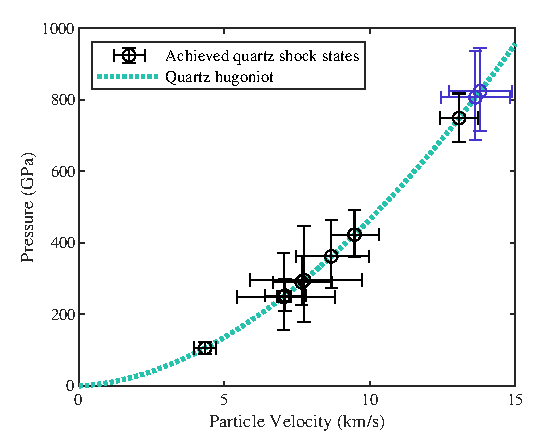
\includegraphics[width=0.6\textwidth]{figures/Experiment/QuartzShockStates_edit.eps}% Here is how to import EPS art
\caption{\label{fig:QuartzShockStates} The quartz shock states achieved in the experimental shots, for the main data set (black) and two additional shots where the quartz signal could be determined with confidence (blue). The shock pressures and particle velocities are calculated based on the quartz hugoniot, and thus all lie exactly on this curve.}
\end{centering}
\end{figure}

This weaker than expected quartz shock strength potentially explains two of the behaviours noted during the experiment. Firstly, the weaker shock will have a lower shock velocity, which explains the longer than predicted shock transit times. Secondly,  many of the shots in Figure \ref{fig:QuartzShockStates} are at pressures around 200-300 GPa, which (particularly when the error range is considered) are comparable to the threshold pressure at which the quartz is expected to become reflective. This provides a potential explanation for the lack of fringe curvature exhibited on the VISAR in most shots; it could well be that the shock pressure simply wasn't high enough for the shock front to exhibit sufficiently high reflectivity. 

A small number of shots in this experiment did demonstrate some degree of fringe curvature, although the weak signal strength meant this couldn't be analysed to a sufficient level for velocities to be determined. It is useful to compare these shots with Figure \ref{fig:PreExpHydro} to check the pressure that this occurred at. Figure \ref{fig:QuartzShockStates} displays 10 shots in total; of these 4 displayed some degree of curvature, at pressures of 290 \unit{\giga\pascal}, 360 \unit{\giga\pascal}, 810 \unit{\giga\pascal} and 820 \unit{\giga\pascal}. There were only 2 shots with pressures above 290 \unit{\giga\pascal} that did not display any curvature (at 450 \unit{\giga\pascal} and 720 \unit{\giga\pascal}). No shots displayed curvature for pressures below 290 \unit{\giga\pascal}. This suggests that it may indeed have been necessary to achieve a pressure above 290 \unit{\giga\pascal} in order to obtain sufficient reflectivity for the VISAR, and thus that the lack of fringe curvature observed on the other shots was likely just a result of the shock pressure being too low. This correlation between the pressure and the shots displaying fringe curvature gives confidence that the shock velocity measurements and calculation of shock pressure are likely accurate.

\subsection{Calculation of velocity from VISAR fringe curvature}

The intention for this experiment was that the VISAR signal would display fringe motion in the quartz, and the quartz shock velocity as a function of time could thus be obtained following the analysis procedure described in Appendix \ref{appdx: VISAR analysis}. Unfortunately this was not possible; very few shots displayed any fringe motion, and those that did had low signal strength or were too noisy for meaningful analysis to be conducted. However, attempts were made to produce such an analysis for shots where some curvature was observed. This was performed based on code written by Dan Eakins, which I adapted for use in this experiment\footnote{In particular, I adapted the code so that it could be used in cases where there were fringe discontinuities which could increase the velocity by an integer number of VPF. I also adapted it so that the code could be used on data where there were only small regions where the fringe signal strength was sufficient for analysis.}.

\begin{figure} [h]
\begin{centering}
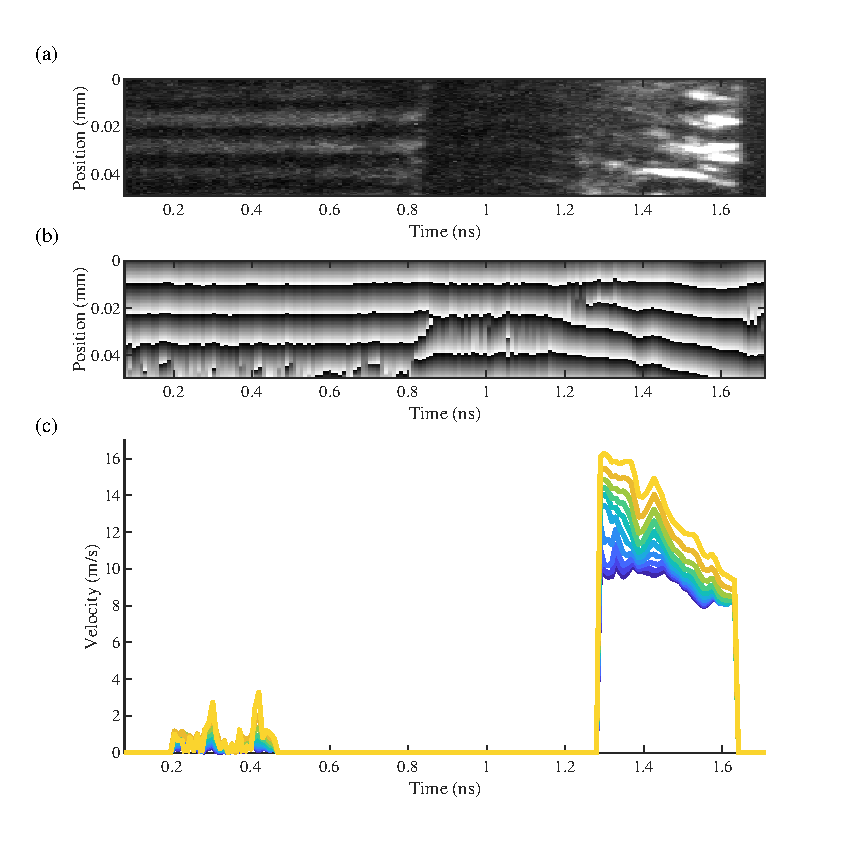
\includegraphics[width=0.8\textwidth]{figures/Experiment/VISARdata.eps}% Here is how to import EPS art
\caption{\label{fig:VISAR curvature analysis} Analsyis of the curved VISAR fringes in shot 39. In a), the fringes in the quartz for the SOP image (cropped and rotated) are shown. In b), the phase has been extracted from this image. The lineouts in c) then show the velocity extracted from these fringes at different vertical positions in the image. The velocity calculation has only included the time period where the fringes are strongest, as including earlier times leads to erraneous results.}
\end{centering}
\end{figure}

Figure \ref{fig:VISAR curvature analysis} shows this analysis for data from shot 39; the only shot in the final data set to show significant curvature. Figure \ref{fig:VISAR curvature analysis} (a) shows the raw VISAR data up until the time of quartz breakout, where it can be seen that the fringes have clearly curved and shifted from their original position. Figure \ref{fig:VISAR curvature analysis} (b) shows this data after filtering has been applied. Here the fringe movement can be seen more clearly; but it is also clear that the low signal leads to discontinuities. In particular, there are regions in the original data where the signal strength is low, and the filtered image is obviously also very poor in these positions. The signal between roughly 1.3 ns and 1.6ns is stronger and produces clearer fringes; this range has been selected, and the analysis applied to allow velocity to be determined from these fringes (relative to the original `zero velocity' fringes before the shock enters the quartz.

Figure \ref{fig:VISAR curvature analysis} (c) then shows velocity traces for different positions within the image according to this reason. As only one VISAR returned a curved signal, it was not possible to unambiguously determine the velocity. As such, the average velocity measurement was used to determine the appropriate integer multiples of the VPF to add to the velocity signal (for this shot, VPF was 8.85 \unit{\meter\per\second}).

The measured average quartz velocity for this shot was $15.8 \pm 1.8$ \unit{\meter\per\second}, and it can be seen that the velocity measured on the VISAR is roughly compatible with this. The trend in velocity seems to vary significantly along the target; the darker traces (corresponding to higher positions in the image) suggest a shock which is reasonably steady, whereas the lighter colors suggest a significant amount of shock decay (this can also be seen by the different amounts of curvature in the fringes in the filtered image). It is unlikely that such a discrepancy in shock behaviour was actually being recorded in the target, particularly as shock breakout (which occurs on the right of the image) is seen to occur at the same time at all positions. This discrepancy is likely due to the poor signal strength - the data is clearly very noisy, and the fringes are much less prominent than would be desired. This analysis therefore shows that the VISAR could in principle be used for such measurements, and the agreement with the average velocity lends a small amount of confidence to this approach; but it is also clear that even for one of the best examples of curved fringes achieved in the experiment the signal was too poor to return useful results, and it is thus difficult to make any conclusions about the shock velocity or stability from this data.




\section{Analysis of SOP data} \label{SOP analysis}


\subsection{Calculating grey-body temperature from SOP data}
As for the VISAR streak images, the x-dimension in the SOP streak image was spatial, while the y-dimension was temporal. The streak time for the camera on each shot was used to convert pixels in the y-direction into time values. An example SOP streak camera image (for the same shot considered in the previous sections) is displayed in Figure \ref{fig:SOP data}

\begin{figure} [h]
\begin{centering}
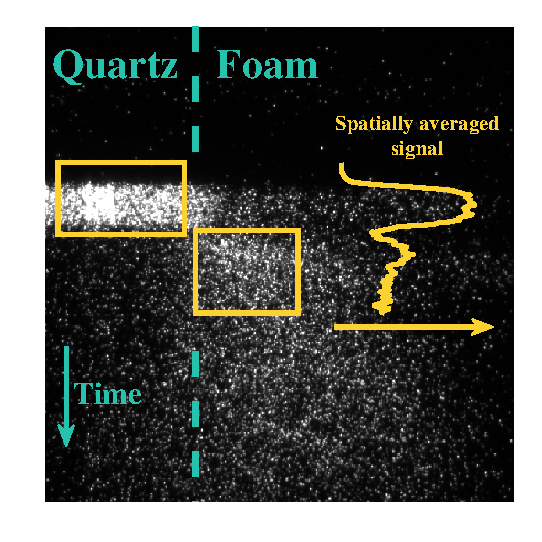
\includegraphics[width=0.6\textwidth]{figures/Experiment/SOPImage.eps}% Here is how to import EPS art
\caption{\label{fig:SOP data} SOP streak image for shot 38. As with the VISAR image, the quartz is positioned on the left of the image, with the foam on the right. Time increased in the negative y-direction. The yellow rectangles represent the chosen regions covering the SOP emission for both materials, while the trace shows the spatially averaged signal across these regions.}
\end{centering}
\end{figure}

In each image, a region was selected covering the emission from the two materials. This region was used for spatial averaging of the signal, to obtain an average intensity vs time for each material; this was chosen to cover the section of the image where the emission was uniform (i.e. to avoid including weaker signal in the averaging from the edge of the target), while being as wide as possible to improve the averaging. The maximum in the averaged signal for the two materials were then identified, and used in the temperature calculation. The selected regions for each material in Figure \ref{fig:SOP data} are indicated by the orange rectangles. As no temporal averaging occurs and only the maximum intensity is used, the temporal range of these selections is not significant; the only concern is ensuring that both peaks are captured, and that the foam selection does not capture any quartz signal (as this would be higher intensity than the foam signal).

In order to calculate the grey-body temperature using Equation \ref{eqn: SOP eqn}, the reflectivity of the two materials was required. This was not measured in the experiment, and thus need to be estimated from other sources. The quartz is a well-characterised reference, and thus relationships between shock velocity and reflectivity have been previously published. The equation \begin{equation} \label{eqn:QuartzR} R_{532} = \num{4.614e-3} + \frac{ (0.3073 - \num{4.614e-3})\cdot U_s^{9.730}}{U_s^{9.730} + 16.185^{9.730}}, \end{equation} published in \cite{Millot2015}, was used to estimate the quartz reflectivity using the shock velocity values determined from the VISAR.

Less literature data exists for the foam. The only relevant data available was for polystyrene \cite{Hu2014}, but this was for solid density plastic rather than a foam. To improve this, collaborators at the University of Rochester performed density functional theory simulations to calculate the foam reflectivity for the conditions achieved in two separate shots. These were performed using the same method used for the polystyrene data (which they were also responsible for) \cite{Hu2014, Hu2017}. They found that for a density of 1.0906~\unit{\gram\per\centi\meter\cubed} and a temperature of 4.8454~\unit{\kilo\electronvolt}, the reflectivity was 0.227, and for a density of 1.0568~\unit{\gram\per\centi\meter\cubed} and a temperature of 1.9743~\unit{\kilo\electronvolt}, the reflectivity was 0.174. 

There were a few options on how reflectivity should be estimated for the other data points. The most basic method would be to assume a linear relationship between these two points. However, it was clear from the polystyrene data that reflectivity saturated at higher pressures; assuming a similar relationship for the TMPTA foam would mean a linear relationship would therefore overestimate reflectivity at these pressures. Instead, the polystyrene fit was scaled using the two new data points. First, the polystyrene data was extrapolated at low pressures to ensure it covered the full intensity range. It was then scaled and shifted so that it passed through both of the new simulation data points. This gave a linear relationship over most of the pressure range of interest, but ensured that the reflectivity saturated at high pressures. This reflectivity curve (with the two points indicated) can be seen in Figure \ref{fig:Foam Reflectivity}.

\begin{figure} [h]
\begin{centering}
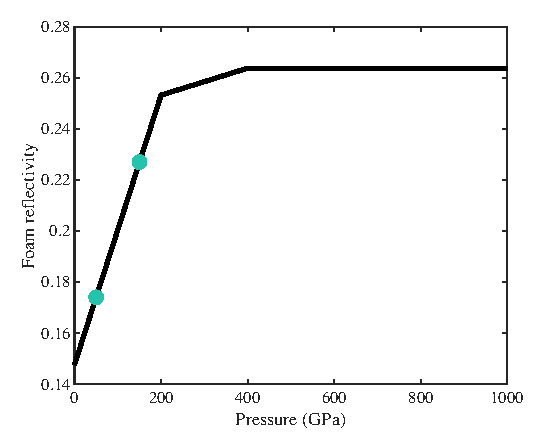
\includegraphics[width=0.6\textwidth]{figures/Experiment/FoamReflectivity.eps}% Here is how to import EPS art
\caption{\label{fig:Foam Reflectivity} The foam reflectivity model used in this work. The polystyrene pressure reflectivity model from \cite{Hu2014} has been scaled so that it passes through the two teal points; these were the results of two DFT simulations for the TMPTA material, performed for this experiment by collaborators at the University of Rochester. It can be seen that for the pressures of interest to this experiment, this is effectively just a linear relationship between the two points. However, this fit ensures that for any MC ransom samples at significantly higher pressures (statistically unlikely), the reflectivity will saturate rather than increasing indefinitely.}
\end{centering}
\end{figure}

As discussed in Section \ref{SOP theory}, the SOP setup was not absolutely calibrated and thus the calibration constant $A$ in Equation \ref{eqn: SOP eqn} could not be determined in advance. The quartz was therefore used as an on-shot temperature reference. Equation \ref{eqn:Temp fit} was used to estimate the expected quartz temperature, based on the the VISAR-determined shock velocity. This temperature and the maximum quartz SOP intensity from the SOP data were substituted into Equation \ref{eqn: SOP eqn} and used to determine $A$. This same calibration constant was then used for the foam data, and the maximum foam intensity was therefore used to calculate the foam shock temperature.

This approach has large uncertainties associated with it. The use of on-shot calibration meant that the quartz temperature had to be estimated, based on the measured quartz shock velocity and fits to previous data; this introduced error that propagated through to the foam temperature. The models to estimate the quartz and foam uncertainty also influence the final result. To capture all these contributors in the final uncertainty quantification, the same Monte Carlo analysis described in \ref{MC error} was applied. The same quartz shock velocity samples used for the impedance matching were also used to perform 10,000 iterations of the temperature calculation. As uncertainties for the various fits used were not quantified, estimates had to be made. The quartz temperature fit was assumed to have an uncertainty of 8\%, as this is the standard uncertainty for SOP temperature measurements at Omega \cite{Millot2015} (where the data for the fit was obtained). The quartz reflectivity fit was assumed to have a 10\% error, based on the size of the error bars in the published data \cite{Millot2015}. The foam reflectivity was given a large error of 0.1, to account for the uncertainty regarding this material (and lack of published experimental data). The streak counts for the quartz and foam measurements were assumed to be based on a Poisson distribution, with the uncertainty appropriate for that distribution used (the square root of the number of counts). The uncertainty in all these models were included in the MC analysis. As described in that section, the quoted temperature for each shot is the `exact' temperature (that obtained without sampling), while the error bars represent the standard deviation of the temperature distributions obtained using the MC methodology.

The results of the temperature measurements, compared to the theoretical modes, are displayed in Figure \ref{fig:SOP Temp}. These results will be discussed in Section \ref{Experiment Results}.

\begin{figure} [h!]
\begin{centering}
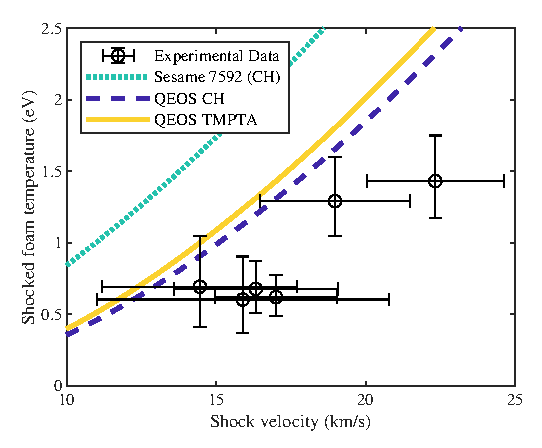
\includegraphics[width=0.6\textwidth]{figures/Experiment/Temp.eps}% Here is how to import EPS art
\caption{\label{fig:SOP Temp} The calculated grey-body temperatures of the shocked foam, as a function of shock velocity, compared to the theoretical equation of state models.}
\end{centering}
\end{figure}

\subsection{Comparing SOP timings to VISAR timings}
It was not possible to identify the breakout timings from each layer directly from the SOP data, as there was no clear change in signal corresponding to shock breakout from the quartz. However, the signal was expected to begin when the shock entered the quartz, and the foam signal was expected to peak at shock breakout from the foam. Based on this, was possible to determine a combined quartz/foam transit time that could be compared to the VISAR data.

This combined transit time for both the SOP and the VISAR data for all the valid experiment shots can be seen in Figure \ref{fig:SOP Timing}. The error bars on the SOP data are large; this is due to the large slit size used for the SOP (used to maximise signal strength), and the large sweep time. However, it can be seen that the agreement between the two diagnostics is good. This comparison serves two purposes. Firstly, it gives more confidence in the timing data for these two shots, as it is confirmed by two independent diagnostics. Secondly, it provides more confidence to the assumption that (despite the relatively low signal strength) the foam peak in the SOP data does in fact correspond to the foam breakout.

\begin{figure} [h!]
\begin{centering}
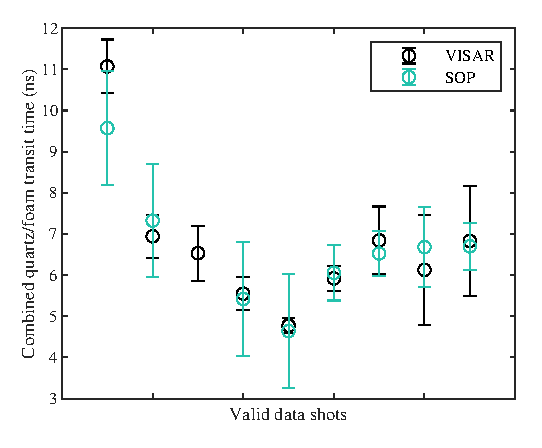
\includegraphics[width=0.6\textwidth]{figures/Experiment/SOPVISARtiming.eps}% Here is how to import EPS art
\caption{\label{fig:SOP Timing} The combined quartz/foam transit time measured using the VISAR (black) and SOP (teal).}
\end{centering}
\end{figure}





\section{Analysis from additional diagnostics} \label{Other diagnostic analysis}

Data was also obtained from the x-ray pinhole camera, fiducial, and photodiode traces of the laser pulse. Firstly, the fiducial allowed the laser switch-on time to be determined, which allowed the shock transit time through the combined ablator and gold layers to be determined. This is discussed in Section \ref{Fidu for coating transit}. The pinhole camera allowed the laser spot size to be estimated, which allowed the assumption of a 400 \unit{\micro\meter} spot to be tested - this is described in Section \ref{Estimating spot size}. Section \ref{Estimating pulse length} describes how the laser pulse length could also be measured (using both the fiducial and photodiode traces). These two pieces of information allowed an estimate of laser intensity to be made; this intensity is then presented in Section \ref{Intensity vs Shock Velocity}, where the trend between laser intensity and shock velocity is also presented. 



\subsection{Using the fiducial to estimate laser turn-on time} \label{Fidu for coating transit}
As discussed in Section \ref{Fidu theory}, a fiducial on one of the VISAR streak cameras displayed the VULCAN pulse, and two-minute shots were performed to allow the time delay between the fiducial and the main pulse to be calculated. Three such shots were performed, and the data from one of these is displayed in Figure \ref{fig:Two Minute}. The time difference between the peak fiducial signal and the peak of the (spatially-averaged) VULCAN signal was calculated. This delay was averaged across the three shots to calculate the `fiducial delay'. 

\begin{figure} [h!]
\begin{centering}
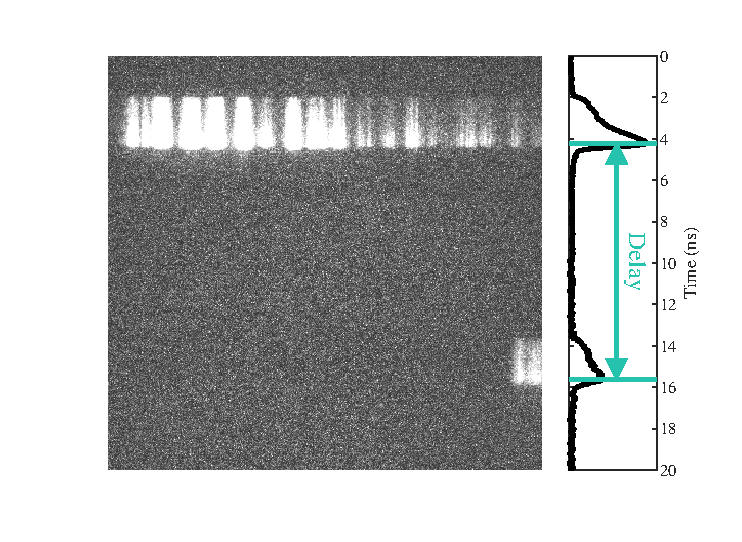
\includegraphics[width=0.7\textwidth]{figures/Experiment/TwoMinute.eps}% Here is how to import EPS art
\caption{\label{fig:Two Minute} VISAR streak for a two minute shot. The main VULCAN signal can be seen, along with the fiducial (on the bottom right of the image). On the right, a lineout is taken showing the average intensity of these signals (the fiducial is averaged only across the pixels where it appears, while the laser signal is averaged across the whole width of the image). The maximum intensity of each of these signals is identified (teal lines), and the delay time between them identified.}
\end{centering}
\end{figure}

The fiducial was not present for many of the early shots. For those where it was present the foot of the fiducial signal was identified, and the previously identified fiducial delay time was subtracted to find the time at which the VULCAN pulse was applied. This had an uncertainty associated with how accurately the fiducial delay could be calculated from the two minute shots, and how accurately the foot of the fiducial could be identified. If the quartz shock entry signal could be identified in the same VISAR streak as the fiducial, it was therefore possible to calculate the ablator/gold transit time - the time between when the laser was first applied and the quartz entry signal. This is shown in Figure \ref{fig:Fidu}. 

\begin{figure} [h]
\begin{centering}
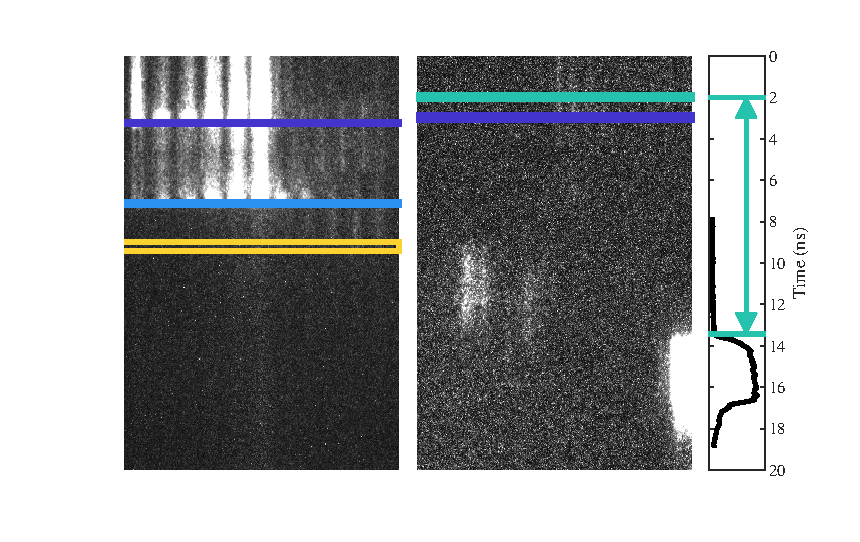
\includegraphics[width=0.9\textwidth]{figures/Experiment/FiduPlot.eps}% Here is how to import EPS art
\caption{\label{fig:Fidu} The two VISAR images for shot 47. The fiducial is present on the second VISAR image. The trace on the right shows the intensity of the fiducial; it's start time is identified, and the delay time is used to estimate when the laser is first applied. This is plotted on the streak image (with uncertainty) in teal. The signal strength on this VISAR image is weak, and only the quartz entry signal (dark blue) is identified; this is sufficient to determine the abltor/gold transit time. The other signals (quartz breakout in light blue, foam breakout in orange) are identified from the other VISAR, where the signal strength is stronger. Shot 47 was used for this figure rather than shot 38, as shot 38 did not include a fiducial.}
\end{centering}
\end{figure}



\subsection{Using the pinhole camera to estimate spot size} \label{Estimating spot size}

The x-ray pinhole camera was used to estimate the laser spot size. This diagnostic was not particularly accurate for such measurements, and was therefore not intended to be used in the intensity calculation; rather, the spot size estimated from this diagnostic could be used to indicate whether the 400 \unit{\micro\meter} spot that the phase plates were desgined to create was in fact being achieved, or if the spot was substantially different from this. It could also be used to identify poor alignment between the six beams. An example pinhole camera image is displayed in Figure \ref{fig:Pinhole Analysis}.

\begin{figure} [h]
\begin{centering}
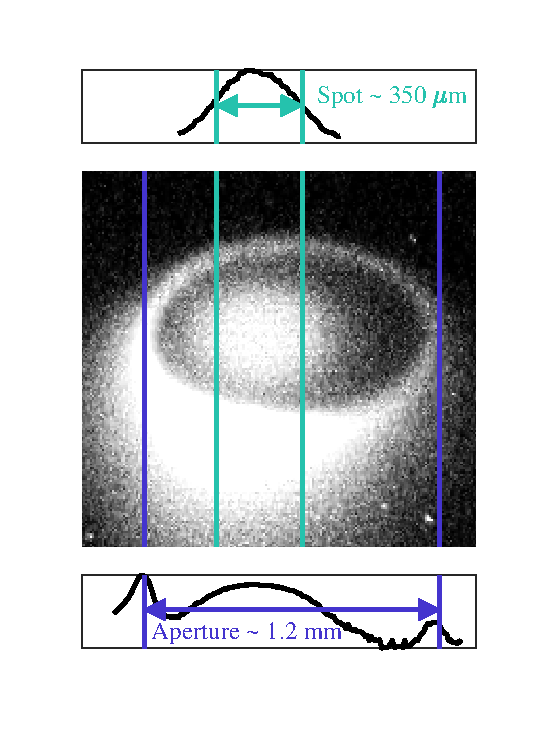
\includegraphics[width=0.6\textwidth]{figures/Experiment/PinholeAnalysis.eps}% Here is how to import EPS art
\caption{\label{fig:Pinhole Analysis} X-ray pinhole image for shot 38. A ring of emission is visible (corresponding to the copper shielding, with a known aperture of $\sim$ 1.2 \unit{\milli\meter} diameter, and the laser spot is visible in the middle of this. The trace below the image shows the log intensity of the signal over a narrow y-range, selected to capture the maximum diameter of the aperture. The position of peak signal either side of the aperture is identified (dark blue lines); this is assumed to be 1.2 \unit{\milli\meter}, providing a reference for the pixel scaling. The trace above the image shows the signal intensity over a narrow region corresponding to the maximum diameter position of the laser spot. The full width half maximum of the spot is then identified (teal lines); in this shot, this was found to be 350 \unit{\micro\meter}.}
\end{centering}
\end{figure}

The pinhole image showed a bright disk corresponding to the laser spot, with a bright halo corresponding to emission from the copper shielding. The fact that the laser seems to be a single spot without noticeable structure suggests good alignment between the six VULCAN beams. As the pinhole camera was positioned above the target the image is distorted in the y-direction, but the camera was normal to the target horizontally and thus the scaling in the x-direction is expected to be accurate. A narrow (in y) region was initially selected, positioned so that the aperture diameter was at it's maximum. The peak in emission either side of the aperture was identified. This can be seen on the trace below the image in Figure \ref{fig:Pinhole Analysis}. The distance between these peaks corresponds to the diameter of the aperture in the copper shielding, which was known to be $\sim$ 1.2 \unit{\milli\meter}. This allowed a horizontal length scale in the image to be determined.

The trace above the image in Figure \ref{fig:Pinhole Analysis} shows the signal in another narrow horizontal selection of the image, located at the peak horizontal diameter of the laser spot. The full-width half-maximum of this signal was identified, and for this shot was measured (using the above scaling) as having a diameter of 350 \unit{\micro\meter}. This method is not expected to give a high accuracy for a variety of reasons (the laser spot clearly extends beyond the FWHM, the diameter of the aperture is assumed etc.) - but the good agreement with the expected 400 \unit{\micro\meter} suggests that the phase plates were producing the desired spot, and thus a spot diameter of 400 \unit{\micro\meter} could reasonably be used for estimating the laser intensity. The pinhole data showed similar good agreement for all relevant shots.

\subsection{Measuring laser pulse length using the fiducial and photodiode traces} \label{Estimating pulse length}

The laser pulse length could be determined using two methods. Firstly, the photodiode traces could be used. Traces were captured for each of the six beams, but these could sometimes include noise/spurious signals. The time and amplitude scales of the traces were also independent, which meant it was not possible to know exactly how the beams varied in strength/timing. Nonetheless, a reasonable estimate of the pulse length could be found by selecting the traces where a sensible signal was recorded, normalising the amplitude of each trace and centring it in time, and then averaging them to produce a combined signal. The pulse length could then be measured as the average full-width half maximum of the individual traces. The six individual laser traces, and the average signal, can be seen in Figure \ref{fig:Fidu and Trace} 

\begin{figure} [h]
\begin{centering}
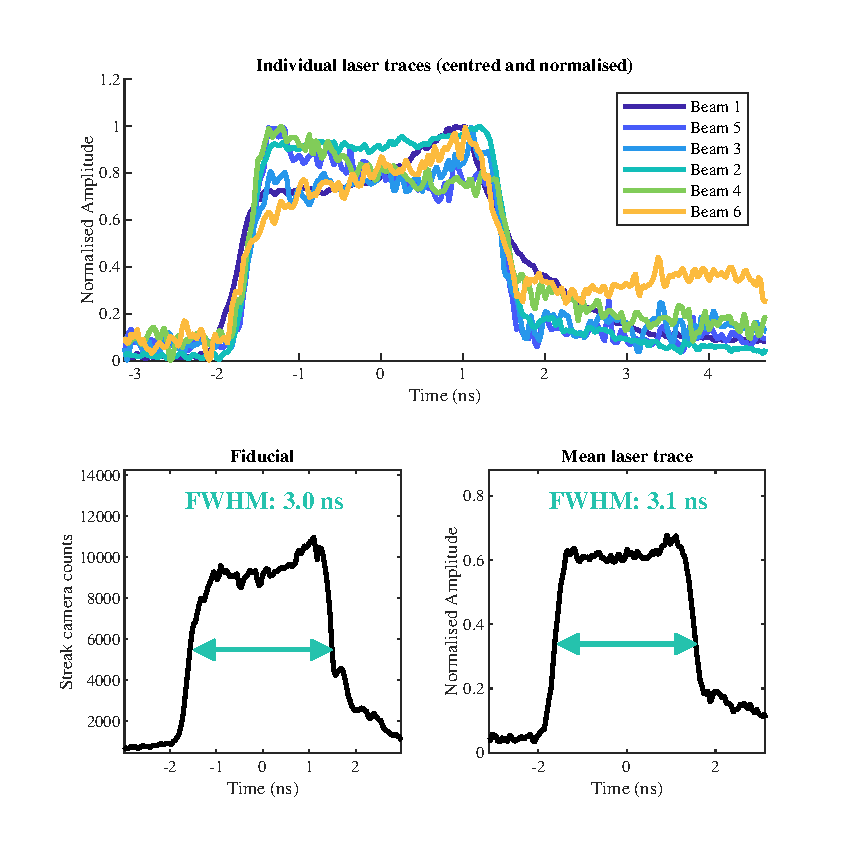
\includegraphics[width=0.8\textwidth]{figures/Experiment/FiduAndTrace.eps}% Here is how to import EPS art
\caption{\label{fig:Fidu and Trace} The laser pulse, as detected using the two methods, for shot 53. The top plot shows the individual traces for the 6 beams, each normalised and centred. The bottom right plot then averages these to approximate the overall pulse. The bottom left plot shows the intensity profile of the fiducial. The fiducial and average pulse traces show good agreement. The full width half maximum of the fiducial and the combined traces also show good agreement, and either can therefore be used to approximate the pulse length.}
\end{centering}
\end{figure}

The fiducial could also be used to measure the pulse length, on shots where this was present and of reasonable intensity. The intensity profile of the fiducial could be extracted from the streak camera image, and also plotted as a function of time. The full-width half maximum of this signal could also be taken and used as a measure of the pulse length. This is also shown in Figure \ref{fig:Fidu and Trace}.

The agreement between these two measures was generally good, as seen in \ref{fig:Fidu and Trace}. It can be seen that averaging the traces also shows a pulse with similar profile to the fiducial, suggesting that both can be used to give a reasonable estimate of the true profile. It was also found that these measured pulse lengths generally agreed well with the pulse length that was requested for the shot. 

Where either the traces or fiducial were present for a shot, the measured pulse length was used in place of the requested pulse length for estimating uncertainty. On shots such as that in Figure \ref{fig:Fidu and Trace} where both were present and the fiducial was of good signal strength the fiducial was used as the more accurate measure, since the fiducial was a measurement of the combined rather than individual beams. The exception to this was for some of the lower intensity shots, where the fiducial strength was much lower; in this case the traces gave a much more detailed and realistic pulse profile, and so these were used instead.

\subsection{Estimating intensity, and comparison with shock strength} \label{Intensity vs Shock Velocity}

The laser energy for each beam was recorded using the on-shot calorimetry. This therefore allowed the laser intensity to be estimated, using the 400 \unit{\micro\meter} spot diameter and the measured pulse lengths. This was performed for each shot.

Figure \ref{fig:Intensity} plots the shock velocity achieved in both the quartz and foam for each shot, as a function of this measured intensity. This provides a simple sanity check on the data; it is expected that the shock strength (and thus shock velocity) in both materials would increase with the laser intensity, and this is indeed the trend seen.

\begin{figure} [h]
\begin{centering}
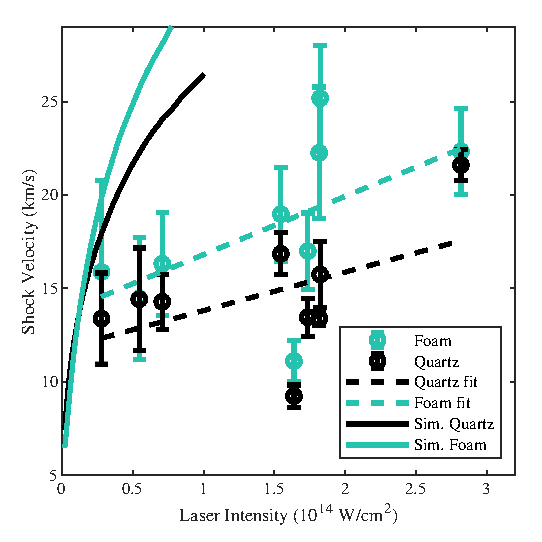
\includegraphics[width=0.6\textwidth]{figures/Experiment/Intensity.eps}% Here is how to import EPS art
\caption{\label{fig:Intensity} The measured shock velocity in the quartz (black) and foam (teal) as a function of intensity. The dashed lines show a linear fit to these two data sets, showing a general trend of increasing shock velocity with intensity. The solid lines show the results from pre-experiment 1D simulations.}
\end{centering}
\end{figure}

Figure \ref{fig:Intensity} also compares this trend to that seen in the pre-shot simulations. This shows a noticeable discrepancy - the shock strength in each material is significantly lower than would be expected in the simulation for a given intensity. This adds to the discussion in Section \ref{Achieved quartz shock states}, where it was observed that the shock pressures achieved in the quartz were significantly lower than had been predicted experimentally. This discrepancy will also be seen in the comparison with post-experiment simulations in Section \ref{Post shock simulations}, and will be explored further in Section \ref{Weak quartz shock}.






\section{Shot selection for final data set} \label{Data choices}

With the main analysis of the data now performed, this final analysis section considers how decisions were made regarding the data set used for the final results. Subsection \ref{Second shock} describes artefacts seen in the VISAR and SOP data on certain shots, and how this is interpreted as potentially corresponding to a shock merger occurring in the quartz. Subsection \ref{Confidence} then outlines the confidence ranking procedure that was used to select shots for the final results, ensuring shots that returned low-quality data or such artefacts were omitted. 

\subsection{Possible evidence of second shocks}\label{Second shock}

A small number of shots showed unexpected additional changes in signal in the VISAR and SOP data. The VISAR data would sometimes display a sudden increase in quartz signal strength part way through the quartz transit time. In the SOP, there would sometimes appear to be distinct periods of emission in the quartz. These two behaviours were often correlated. VISAR and SOP data for a shot where this is observed are displayed in Figure \ref{fig:Second Shock}.

\begin{figure} [h]
\begin{centering}
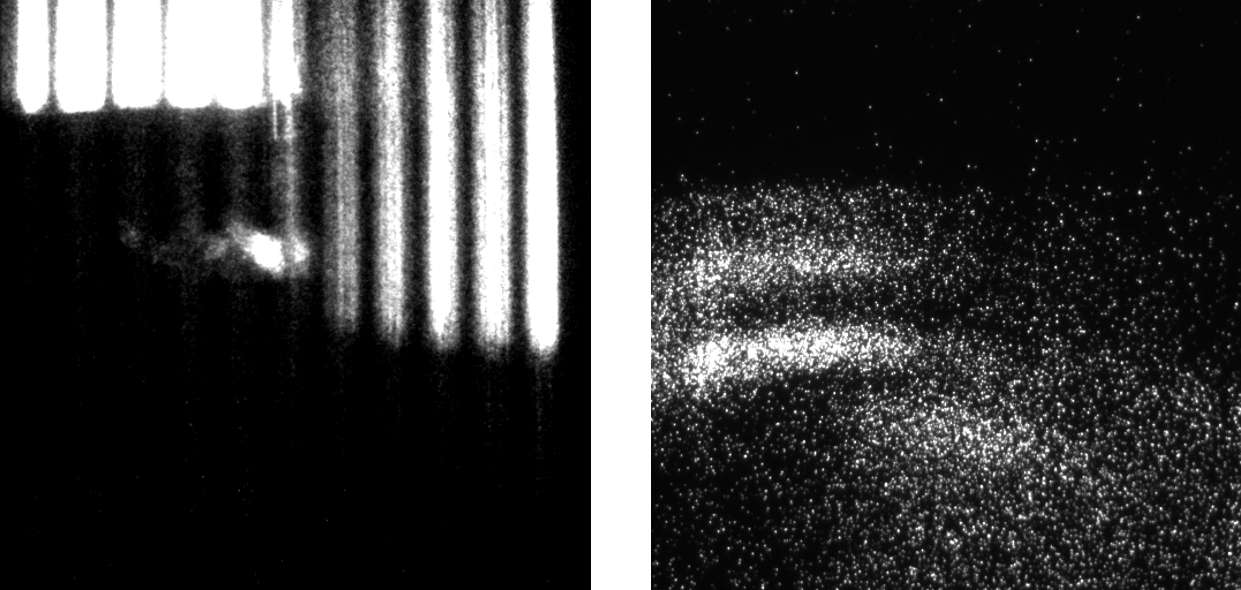
\includegraphics[width=0.8\textwidth]{figures/Experiment/Second Shock.png}% Here is how to import EPS art
\caption{\label{fig:Second Shock} VISAR (left) and SOP (right) data for shot 62, displaying a possible second shock. A sudden increase in the intensity of the VISAR signal is seen as the shock transits the quartz, which could correspond to a higher pressure shock with enhanced reflectivity. In the SOP signal, two distinct bands of emission within the quartz are observed.}
\end{centering}
\end{figure}

The most likely explanation for this would seem to be a second shock, which catches and overtakes the primary shock within the quartz layer. This would lead to a higher shock pressure being achieved in the quartz later in time (and thus an increased reflectivity and large VISAR signal), and an increase in shock temperature (and thus a region of second emission). Such a behaviour would mean that the velocity of the shock front would change during the quartz transit, and thus the calculated average shock velocity would not be physically meaningful. This would prevent an accurate impedance matching calculation from being performed. For this reason, any shots where such behaviour was observed were not included in the final results for this experiment.

The second shock phenomena was observed in the pre-experiment hydrodynamic simulations for higher intensities, and is discussed in Section \ref{Target Design}. The increased quartz thickness used in the experiment (see Section \ref{Target issues}) made this problem more likely, as did the higher intensities used (in an attempt to generate stronger shocks). 

This effect was investigated in post-shot simulations, and is discussed in Section \ref{Shock merger}. These simulations suggested that the second shock could indeed be an issue in this regime, but it was not possible to predict/recreate this behaviour for specific shots. This is a difficult phenomena to simulate - the state behind the first shock is already complicated, and will have some error/uncertainty compared to the real experimental conditions, and thus describing the transit of a second shock through this uncertain state is likely to have much larger uncertainty associated with it. In addition, later sections will demonstrate that there is a discrepancy between the shock strength in the quartz layer seen in the experiment relative to the simulations; such an effect would also impact any secondary shocks, leading to further uncertainty surrounding this effect. By omitting the shots where this behaviour is observed it is assumed that this effect has not had a significant impact on the experimental results; however, it is possible that in some shots the second shock would have undergone recombination in the foam, and this may not lead to an obvious signal.

\subsection{Confidence ranking of shots} \label{Confidence}
Only a fraction of the experimental shots resulted in VISAR images where all three necessary transitions could be confidently identified. Often it was not possible to select a particular breakout time from the VISAR data, or it was unclear if there was really a change in signal there. To account for this, a confidence ranking of each shot was performed as the data was analysed.

Each shot was given a score between 0 and 10. A 10 meant that it was absolutely certain that the times identified corresponded to those signals. A 0 meant that there was no timings which could be determined. A range of factors contributed to this ranking. Agreement between the two VISARs resulted in higher confidence, while unexpected artefacts or behaviours in the signals led to lower confidence (as did unreasonable calculated values). This was an iterative process, which was returned to with later information (such as evidence of second shocks, or cross-comparison with SOP data). For the final results only data with a confidence value greater than 5 were used, which removed shots where there was low confidence that real behaviours were being measured. 


\section{Results and discussion} \label{Experiment Results}

The foam shock states achieved for each shot in the final data set are displayed in Figure \ref{fig:Hugoniot Results}, in the ($u_p,P$) plane. These data points are compared to three theoretical hugoniots generated using different equation of state models; the SESAME EOS for CH \cite{SESAME}, as well as a quotidian EOS (QEOS) model for both CH and TMPTA \cite{More1988}, generated using the HUGONIOT utility packaged with \texttt{HYADES} and provided by Cascade Inc. In each case, the hugoniots are generated for the homogeneous material at the foam density, rather than for a foam material. The QEOS models demonstrate that for the compression behaviour, there is no noticeable difference between CH and TMPTA; and thus it is a reasonable comparison to use the CH SESAME table (there is no TMPTA SESAME table to be compared to).

\begin{figure} [h!]
\begin{centering}
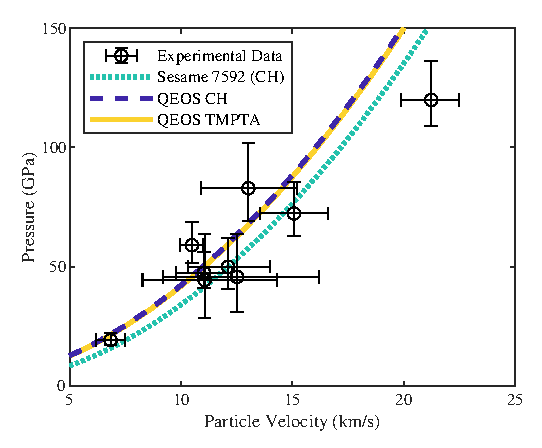
\includegraphics[width=0.6\textwidth]{figures/Experiment/Hugoniot.eps}% Here is how to import EPS art
\caption{\label{fig:Hugoniot Results} The calculated grey-body temperatures of the shocked foam, as a function of shock velocity, compared to the theoretical equation of state models.}
\end{centering}
\end{figure}

The data is well described by all three of the models, although the large error bars unfortunately prevent a conclusion being drawn about which model provides the best fit. As is expected, the error is dominated by the experimental uncertainty in the quartz and foam shock velocities (with the hugoniot error for instance contributing very little). It can be seen that the highest pressure point is not well described by any of the three models, and is at significantly lower pressure than these models predict. This could be indicative that the models describe the material less well at high pressure; however, it is not possible to make any conclusions about this based on a single data point.

Overall, this suggests that in the pressure range displayed in Figure \ref{fig:Hugoniot Results}, the three theoretical models used here are sufficient to describe the material to within the experimental uncertainty. This is notable due to the fact that they are based on the homogeneous material; and this therefore suggests that this approximation is a valid one to this level of uncertainty for this material. This is a useful result, as it means that such foams should therefore be able to be simulated to reasonable accuracies using these models, rather than requiring foam specific versions.

The grey-body foam temperature is displayed in Figure \ref{fig:SOP Temp Results}. There are fewer data points on this plot, as the SOP did not return good data for all the shots shown in Figure \ref{fig:Hugoniot Results}. Here, it is clear that the theoretical models do not well describe the experimental data; all three theoretical models pass above all of the data points, and many of the data points are outside of the error of these predictions. This is despite the large error bars, which originate from the large experimental uncertainty in the shock velocities, along with the large uncertainty in the foam reflectivity model.

However, there is not sufficient confidence in this temperature data to make firm conclusions about the accuracy of the theoretical models. As noted previously, the SOP signal in this experiment was very weak; it was often difficult to detect any foam signal, and the streak camera had to be operated on maximum gain. As such, this temperature data should be used as an initial indication of this only; it may well be that there is a temperature difference from the models, but this would need to be explored with more accurate temperature measurements before this could be concluded with any degree of certainty.

\begin{figure} [h!]
\begin{centering}
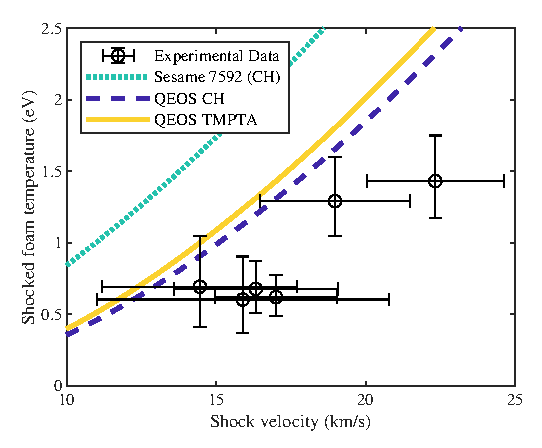
\includegraphics[width=0.6\textwidth]{figures/Experiment/Temp.eps}% Here is how to import EPS art
\caption{\label{fig:SOP Temp Results} The calculated grey-body temperatures of the shocked foam, as a function of shock velocity, compared to the theoretical equation of state models.}
\end{centering}
\end{figure}

These experimental results can be compared with those obtained in previous experiments, looking at similar materials. In particular, the data here is compared to the results of explosively driven experiments performed at Los Alamos on CH foams \cite{Marsh1980}, absolute Hugoniot  measurements of CH foam performed using the Naval Research Laboratory's Nike Laser facility \cite{Aglitskiy2018}, and impedance matched TMPTA-plastic foam experiments performed at the LULI facility at Ecole Polytechnique \cite{Koenig1999}. These experiments explored foams at a range of densities, which leads to an interesting comparison - as seen in Figure \ref{fig:Other Foam Data}.

\begin{figure} [h!]
\begin{centering}
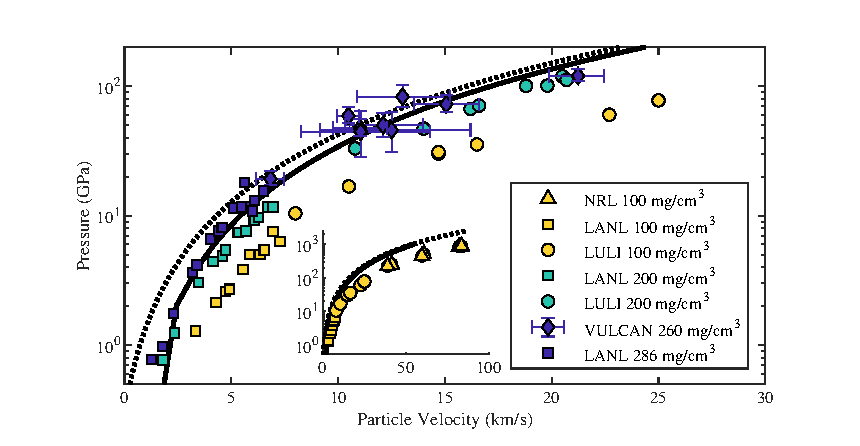
\includegraphics[width=1.0\textwidth]{figures/Experiment/OtherDataUpP_wide.eps}% Here is how to import EPS art
\caption{\label{fig:Other Foam Data} A comparison of the experimental data points with CH and TMPTA data from previous experiments. The different colours represent different initial densities, while the different symbols represent the facility they were performed at. The NRL data has a much larger particle velocity than the other experiments, and thus is not visible on the main plot; the inset therefore shows the 100 \unit{\milli\gram\per\centi\meter\cubed} data over a wider velocity range to include these results. }
\end{centering}
\end{figure}

In a plot of ($U_p,P$), as seen in Figure \ref{fig:Other Foam Data}, the Hugoniot dependence on density is observed. For higher initial density foams (darker colours in the figure), the experimentally achieved pressure is higher. There are three rough density groupings in the figure, and as expected it can be seen that the data groups into three curves based on this. This trend is consistent between data sets and facilities, and is seen across the full pressure range investigated.

The SESAME and QEOS Hugoniots for CH used in Figure \ref{fig:Hugoniot Results} are also repeated here. It can be seen that the LANL data for a similar initial density (slightly higher at 286 \unit{\milli\gram\per\centi\meter\cubed}) continues the trend seen in the data from this experiment at lower pressures, effectively extending the pressure range of the data set to cover two orders of magnitude. It can be seen that both experimental models capture the rough trend of the data over this range, but the SESAME model appears to match the LANL data at low pressure more closely than the QEOS model, potentially suggesting that the SESAME model better describes these foams over the wider pressure range.

\begin{figure} [h!]
\begin{centering}
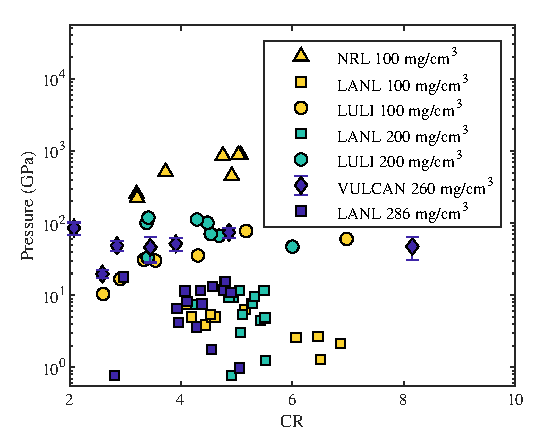
\includegraphics[width=0.6\textwidth]{figures/Experiment/OtherDataCR.eps}% Here is how to import EPS art
\caption{\label{fig:Other Foam Data CR} A comparison between the different experiments, but in terms of the compression ratio. Horizontal error bars have been emitted as they cover the full horizontal range of the plot. No trends are obvious given the spread of the data. }
\end{centering}
\end{figure}

The same data could also be considered in terms of compression ratio vs pressure, where compression ratio is the density of the shocked material divided by it's initial density. This is displayed in Figure \ref{fig:Other Foam Data CR}. However, density is particularly sensitive to the uncertainty in the data, leading to large relative errors in this value \cite{LePape2008}. For this reason error bars are not displayed on this plot for clarity, as they cover the full horizontal range. This issue also affects the other experiments, and makes discrimination between models impossible even with the addition of the new data set.











\section{Comparison with simulation} \label{Post shock simulations}

Post-experiment simulations were also performed in a variety of 1D and 2D codes in order to compare with and help interpret the experimental results. These simulations used the real measured target dimensions. A realistic laser profile was used; the intensity profile of the fiducial was normalised, and scaled to give the appropriate laser intensity (as seen in Section \ref{Estimating pulse length}, the fiducial trace was seen to show good agreement with the photodiode traces and thus gave a reasonable approximation of the pulse). Such simulations were performed in the codes \texttt{HYADES} (by the author), \texttt{HELIOS} (seperately by both the author, and by Artem Martynenko and Paul Neumayer), \texttt{MULTI} (by Artem Martynenko and Paul Neumayer), and \texttt{FLASH} (by Piotr R\k{a}czka).

An example 2D \texttt{FLASH} simulation (performed by Piotr R\k{a}czka) is displayed in Figure \ref{fig:SimSubPlot}. The 2D \texttt{FLASH} simulations are unique as the only ones to include the 2D step structure, and were thus used to assess the impact of the step on shock propagation. In Figure \ref{fig:SimSubPlot} (a), the 2D shock is displayed at four snapshots in time. The step structure is seen to have no significant effect on the shock; the target has a planar shock front across the majority of the laser spot, and this is not significantly disrupted by the presence of the step. The shock propagation as a function of time at a particular horizontal position within the target is displayed in Figure \ref{fig:SimSubPlot} (b), allowing the shock transit times through the target to be determined.

Three key features of the post-experiment simulations will be discussed in this section. First, the shock propagation times will be compared between experiment and simulation. Second, the level of shock stability will be investigated. Finally, the shock merger pheonema will be discussed.

\begin{figure*} [h!]
\begin{centering}
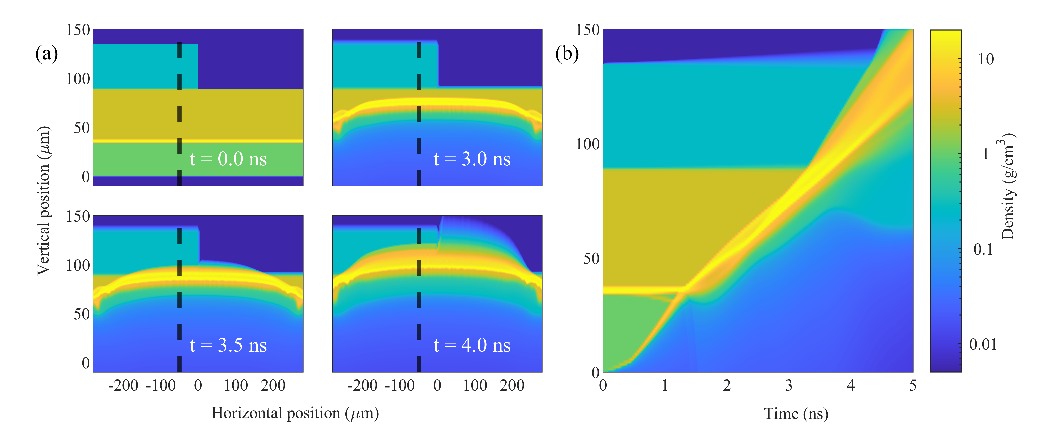
\includegraphics[width=1\textwidth]{figures/Experiment/SimSubPlot.eps}% Here is how to import EPS art
\caption{\label{fig:SimSubPlot} 2D \texttt{FLASH} simulation (performed by Piotr R\k{a}czka) using the measured target dimensions and temporal laser profile for shot 47, with a peak simulated laser intensity of \num{1.8E14} \si[per-mode=symbol]{W/cm^2}. (a) shows four snapshots of the shock propagating through the target in 2D. It can be seen that the shock propagation through the foam is largely undisturbed by the step structure. (b) shows the shock propagation vs time at a single horizontal position (50 \si[per-mode=symbol]{\micro\meter} within the target, indicated by the dashed black line in (a). The same colour scale (representing density) is used in all plots.}
\end{centering}
\end{figure*}

\subsection{Shock propagation time} \label{Shock propagation time}

Simulations were performed in all of these aforementioned codes for shot 47 for a range of laser intensities and thus shock strengths. The same realistic laser profile was used, but scaled to different maximum intensities. For each simulation, the transit time of the shock through the ablator/gold and quartz layers was measured. These timings were compared to the experimentally measured transit times for these layers (determined from the VISAR for the quartz, and from the fiducial for the ablator/gold); this can be seen in Figure \ref{fig:SimulationPlot}. The figure shows good agreement between the different codes (both 1D and 2D) for these propagation times. 

\begin{figure} [h!]
\begin{centering}
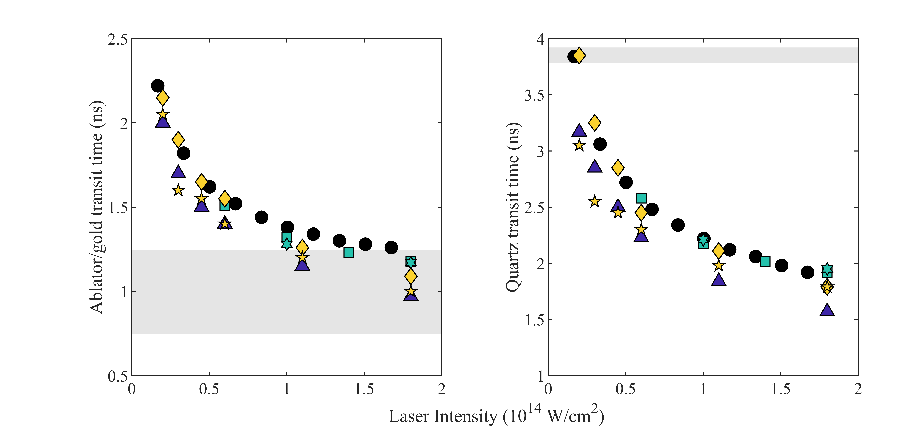
\includegraphics{figures/Experiment/SimulationVertical_edit.eps}% Here is how to import EPS art
\caption{\label{fig:SimulationPlot} Simulated shock transit times through the combined ablator/gold layers (left) and the quartz layer (right) for shot 47. This was performed in four different 1D radiation hydrodynamics codes: \texttt{HYADES} (black circles), \texttt{FLASH} (teal squares), \texttt{MULTI} (yellow diamonds) and \texttt{HELIOS} (blue triangles). 2D simulations were also performed in \texttt{MULTI} (yellow stars) and \texttt{FLASH} (teal hexagrams). On each plot, the grey shaded region corresponds to the experimentally measured value (bounded by the uncertainty). The agreement between codes is good, but in all cases it is not possible to match the experimentally measured times in both ablator/gold and quartz layers at any one intensity. \texttt{HYADES} simulations here were performed by the author, while those in other codes were performed by collaborators.}
\end{centering}
\end{figure}

It is clear from the figure that it is not possible to match transit times in the two materials in a single simulation (i.e. for a single laser intensity). This was found to be the case for all the targets. Matching the experimentally measured ablator/quartz transit times requires a high intensity, comparable to the $\sim$\num{1.8e14}~\si[per-mode=symbol]{W/cm^2} intensity used in the real shot. However, matching the quartz transit time requires this simulated intensity to be almost an order of magnitude lower. This is a significant discrepancy, and suggests that something is causing the shock to be significantly weaker in the quartz than in previous layers in the target, and than would be expected based on the simulations. 

It was noted throughout the analysis that the quartz shock strength was weaker than expected. This analysis shows that the shock is not weaker across the whole target (i.e. that it is not due to, for instance, a lower than expected laser intensity - something also ruled out by the analysis in Section \ref{Other diagnostic analysis}), but rather due to a decrease in shock strength within the target. This weaker quartz shock also helps provide an explanation for the lack of VISAR fringe curvature, and further supports the claim made in Section \ref{Achieved quartz shock states} that this was due to an insufficient quartz shock pressure. This discrepancy between the shock strength in the ablator/gold and the quartz will be further discussed and investigated in Section \ref{Weak quartz shock}, where a possible mechanism will be proposed and explored.

It is important to note at this point that this effect does not affect the accuracy of the impedance matching calculation, and thus does not undermine the previously presented results. This calculation simply requires that a shock passes through the quartz and into the foam, and that it is reasonably consistent across these two layers; the fact that the shock was previously stronger in the ablator/gold layers is not significant. The shock velocity measurements are not made until the shock has entered the quartz, and thus the shock behaviour in the previous layers is not captured\footnote{Of course, the exception here would be if whatever is responsible for this decrease in shock strength led to other effects, such as significant shock decay beyond that seen in the simulation. These second order effects could influence the impedance matching calculation. However, no evidence for such effects was observed}.

\subsection{Shock stability}

The simulations also allowed the stability of the shock to be investigated. The impedance matching calculation requires accurate knowledge of the shock either side of the interface - the shock velocity immediately before it exits the quartz, and immediately after it enters the foam. Yet in this experiment average shock velocities for these two materials were used\footnote{Had the VISAR data displayed sufficient fringe curvature for the quartz shock velocity to be determined as a function of time, the shock stability would be known and the shock velocity could be determined just prior to shock breakout.}, and thus the calculation therefore requires that the shock is reasonably stable (without significant decay) within these two layers. Any deviation from a stable shock would introduce a systematic error.

\begin{figure} [h!]
\begin{centering}
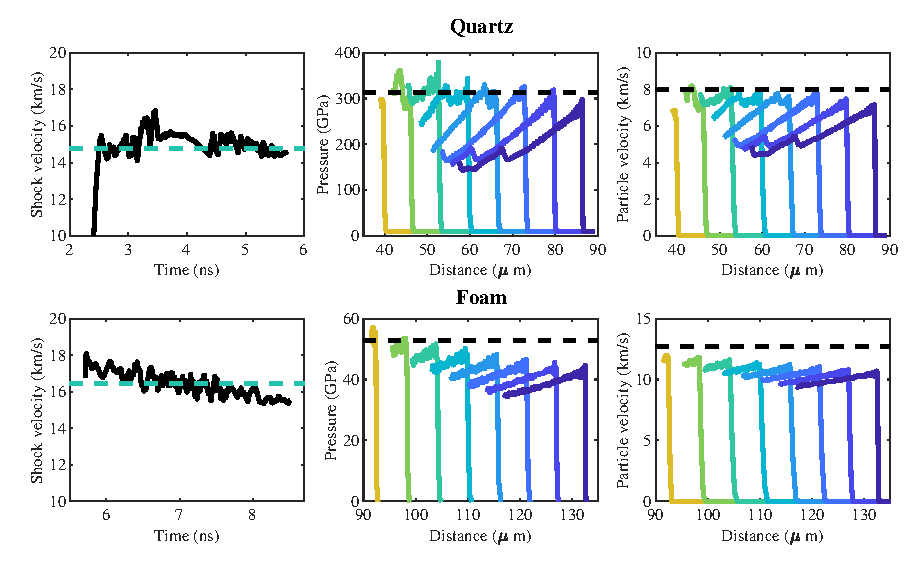
\includegraphics[width=1\textwidth]{figures/Experiment/ShockDecay_wide.eps}% Here is how to import EPS art
\caption{\label{fig:ShockDecay} Simulated shock velocity, pressure and particle velocity at the shock front as the shock propagates through the quartz and foam layers, from a 1D \texttt{HELIOS} simulation (performed by the author) of shot 47 with a simulated laser intensity of \num{1.5E13} \si[per-mode=symbol]{W/cm^2}. The shock velocity is displayed as a function of time, while for pressure and particle velocity, profiles of the shock front are provided at eight equally spaced time intervals (later times are further to the right, and are plotted in darker colour). The shock transit times through the quartz and the foam were used to calculate average shock velocities (the dashed horizontal teal lines). The same analysis procedure as used on the experimental data was then used to calculate the pressure and particle velocity in the two materials (the dashed horizontal black lines).}
\end{centering}
\end{figure}

Figure \ref{fig:ShockDecay} shows the simulated shock velocity, pressure, and particle velocity in the foam from a 1D \texttt{HELIOS} simulation, again using the realistic laser profile. While the shock is relatively stable, a small amount of decay is seen in both materials. This is most significant in the foam shock pressure. The dashed teal line in the shock velocity plots indicates the average shock velocity which would be calculated for each layer based on the shock propagation time, representing the value which would be measured experimentally. The impedance matching calculation was then performed for these two average velocity measurements, and the results of this are represented by the dashed black lines in the pressure and particle velocity plots; these represent the values that would be calculated based on these experimental results. Ideally, these should correspond to the shock state just before the shock leaves the quartz (the darkest trace in the quartz plots) and just after it enters the foam (the lightest foam trace). In the case of Figure \ref{fig:ShockDecay} it can be seen that the shock decay does indeed lead to some discrepancy, but this is relatively small and the calculated values are a reasonable approximation of these shock states. Indeed, this suggests that the use of average shock velocities in this experiment was sufficient to give calculated shock states average to within a systematic error (based on the shock decay) of around 10\%, which is reasonable and typically less than the random error represented by the error bars in the experimental data.

\subsection{Shock merger} \label{Shock merger}

A second potential systematic error was the second shock which originates in the gold layer, reflects from the ablation front, and could potentially merge with the primary shock within the quartz or foam layers. The experiment was designed to mitigate this phenomena through choice of target dimensions and laser intensities, as discussed in Section \ref{Target Design}. However, the delivered targets were often thicker than originally proposed, and the low shock strength led to larger laser intensities being frequently used. Both of these effects made the second shock more probable. Section \ref{Second shock} described how some of the experimental shots appeared to indicate that this shock merger had occurred in the quartz, and were thus not included in the final data set.

Simulations were performed for some of the shots where a second shock was seen to occur in the data, using the real laser profiles; however, these did not recreate the observed behaviour. Meanwhile, many of the higher intensity simulations of shots which did not appear to show this effect did demonstrate it. This can be seen in Figure \ref{fig:ShockPlot}, which shows the propagation of shots through the Lagrangian simulation zones of the target in a 1D \texttt{HYADES} simulation. It can be clearly seen here that the second shock merges with the first just as it crosses from the quartz into the foam. This effect was found to be different between codes; the 2D \texttt{FLASH} simulation shown in Figure \ref{fig:ShockDecay} of the same shot shows the merger occurring earlier in the quartz, while in a 1D \texttt{HELIOS} simulation with the same settings the merger does not occur until the shock breaks out from the rear of the target.

\begin{figure}
\begin{centering}
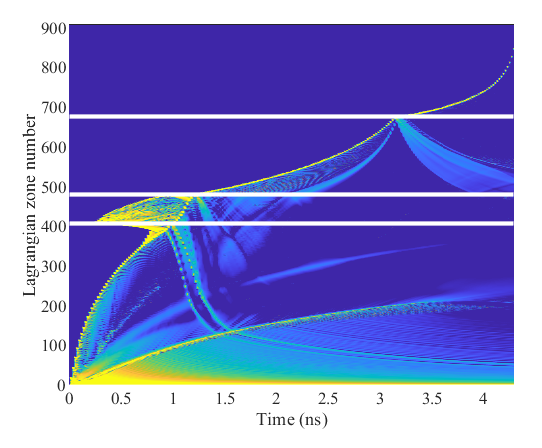
\includegraphics{figures/Experiment/ShockPlot2.eps}% Here is how to import EPS art
\caption{\label{fig:ShockPlot} Shock propagation plot (log derivative of pressure) from a 1D \texttt{HYADES} simulation of the same shot (47) and laser intensity as in Figure \ref{fig:SimSubPlot}. It can be seen that a second shock (originating from the gold layer) catches and overtakes the primary shock just before it reaches the foam layer (this is different to the \texttt{FLASH} simulation, where this occurs at an earlier time). The figure is plotted as a function of Lagrangian simulation zone number (rather than radius), so that the zone material boundaries are stationary and the shock propagation can be seen more easily. The material interfaces are indicated by the white horizontal lines.}
\end{centering}
\end{figure}

This difference between codes demonstrates the difficulty in accurately simulating this effect. The second shock has a particularly large uncertainty associated with it, as it is propagating through material which has already been shocked. Any uncertainty/difference between codes in the first shock will result in a different shock state for this first material, which will then be magnified further with the transit of the second shock. In addition to this, Section \ref{Shock propagation time} already noted that the simulations cannot accurately describe the shock propagation through the target in a single simulation, as there is an unexplained decrease in shock strength between the ablator/gold. This effect would also be expected to have a significant (but unknown) impact on the second shock, which would also not be included in the simulations. Given this, it is no surprise that it is not possible to simulate accurately whether this effect will or will not occur for a given shot. It is expected that by identifying shots which show behaviour linked to this effect, as described in Section \ref{Second shock}, this shock merger should not have had a significant impact on the experimental results (although it is worth noting that it may not be possible to identify cases where the shock merger occurred within the foam layer).

\section{Investigation of the shock strength discrepancy} \label{Weak quartz shock}

Throughout the analysis section it was noted that the shock strength seen in the experiment was significantly lower than predicted in the simulations performed prior to the experiment. This was further highlighted by the post-experiment simulations, which also suggested that the shock strength in the ablator/gold layers was much closer to the simulated results - suggesting that something was leading to a decrease in shock strength between these two layers. This section presents some further investigation of this discrepancy, and proposes a potential explanation.

\subsection{Analysis of non-data targets} \label{Non-data targets}

As discussed in Section \ref{Target issues}, in some of the early targets the gold/CH coating delaminated from the quartz, and had to be glued back on. The resulting glue layer between the quartz and gold layers prevented the average quartz transit time from being accurately measured, which meant that the quartz shock state could not be determined and thus impedance matching could not be performed. These targets were shot early on as setup targets while first testing the system. 

A disproportionate number of these glue targets displayed fringe curvature compared to the data targets. There were 5 glue targets shot, and three of these displayed clear evidence of curvature. Of the other two, one displayed no clear signal at all, and in the other it was not possible to determine if there was curvature or not. This is a much better success rate than for targets without glue - 38 of these targets were shot in total, and only 7 displayed any signs of possible fringe motion. 

As discussed in Section \ref{Achieved quartz shock states}, fringe curvature in this experiment generally correlated to a higher quartz pressure, and this suggests that the glue targets were far more likely to access higher pressures in this experiment than targets without glue. As the targets were otherwise alike, this suggests that gluing the gold and quartz together tended to improve the shock strength in the quartz - which in turn suggests that the decrease in shock strength might be arising at the interface between these two materials.

%An aluminium reference target was also shot during the experimental campaign, consisting of a single piece of aluminium with a step machined in it (and thus no coating or different layers). This target was simulated, and it was found that it was possible to match the transit time through the two steps of this target in a single simulation (although at a lower intensity than was actually used). This target is much simpler than the data target and so they cannot be compared too closely. However, it does suggest that the shock discrepancy issue originates in the target, rather than in the laser. The fact such a target, without interfaces, can be matched with experiment also is compatible with the discrepancy occurring as the shock crosses from the gold to the quartz.

\subsection{Proposed explanation for the discrepancy} \label{Curvature and Pressure}

The key points are therefore as follows:
\begin{itemize}
    \item The shock decreases significantly in strength between the ablator/gold layers and the quartz layer, compared to 1D and 2D simulation.
    \item This effect is not seen between the quartz and foam layers, suggesting it is not a simple shock decay.
   % \item This effect is not seen in an solid aluminium target.
    \item Gluing the gold to the quartz appears to significantly improve the shock strength in the quartz.
\end{itemize}

The proposed explanation for this behaviour is a poor contact between the gold and quartz layers, which led to a loss of shock strength as the shock crossed this interface. This would likely be a partial delamination between these two layers, resulting in gaps between the two materials. This is something that could well have happened, given that full delamination of these layers was observed in a small number of cases. Gluing the gold on to the quartz would prevent such delamination from occurring, which would explain why adding a glue layer seemed to enable higher shock pressures in the quartz. This is the working assumption for why this discrepancy was occurred, as no other explanation was found that could explain all the aforementioned evidence.


\subsection{Simulation of a gap between layers}

Efforts were made to simulate the impact of a gap between these layers. \texttt{HYADES} simulations were performed using a low gas fill between the layers, or a \texttt{HYADES} `vacuum' zone\footnote{A Lagrangian zone which closes once compressed}, but neither resulted in any reduction in shock strength in the quartz, nor a significant increase in shock transit time. Further simulations performed by collaborators using \texttt{MULTI} and \texttt{FLASH} also failed to find a substantial change in behaviour when a gap was included.

However, it is possible that such an effect could not be captured in one-dimensional hydrodynamics codes. Firstly, there is no obvious energy loss mechanism in 1D, and so once the gold material crosses the gap, the shock would continue undisturbed. This can also be demonstrated by the following simple model. When the shock reaches the rear target surface, it will undergo free surface expansion at roughly twice the shock velocity \cite{Forbes2012}. If this is approximated as a uniform density plate at the shocked density (a very basic assumption, since in fact the expanding gold will have a strong density gradient), then the impact of the gold and quartz can be considered as a standard plate flier impedance match experiment (a commonly discussed setup \cite{Forbes2012}). The solution to this interaction is a shock wave in the quartz with the exact same strength as if there had been no gap.

However, it is suggested that in a real interaction, there may be more losses. The shock will not be perfectly planar or uniform, and this will be exacerbated by the material crossing the gap. There could also be lateral energy transfer during this process. The process of shock-breakout is likely not perfectly clean and ideal, and all these factors could contribute to a reduction in the shock strength.

This was investigated in a series of 2D simulations, performed by Piotr R\k{a}czka in a customised version of \texttt{FLASH} (since \texttt{FLASH} does not natively support non-linear boundaries). Three different gaps were simulated with varying degrees of non-uniformity, as seen in Figure \ref{fig:GapSims}. The level of non-uniformity in the gap does appear to correlate with an increased shock propagation time. However, this is a very small increase, on the order of tens of picoseconds, and is thus significantly smaller than the nanosecond level discrepancy seen previously. As such, the simulated behaviour clearly not explain this effect. However, it is worth noting that a real gap would likely be highly non-linear, and thus it is possible that this effect could be much greater in magnitude in practice.

\begin{figure} [h!]
\begin{centering}
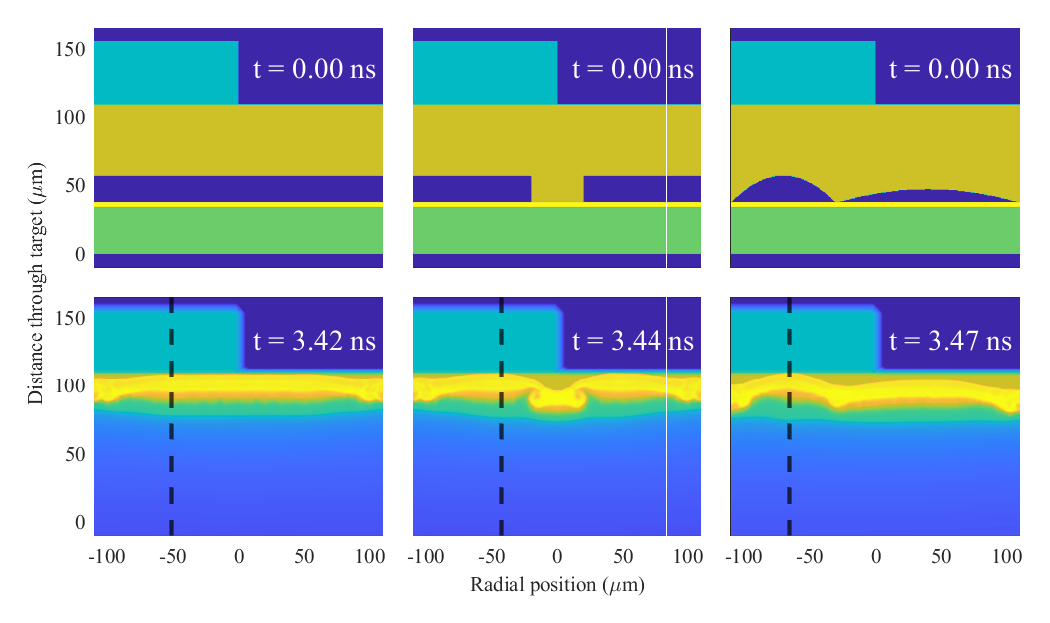
\includegraphics[width=1\textwidth]{figures/Experiment/GapSims.eps}% Here is how to import EPS art
\caption{\label{fig:GapSims} 2D of three different gap structures in \texttt{FLASH}, performed by Piotr R\k{a}czka. The bottom row of plots show the time at which the shock front first breaks out from the quartz, while the dashed black line indicates the position this occurs at. Increasing the non-linearity of this gap structure is shown to increase the propagation time, albeit by a small amount.}
\end{centering}
\end{figure}

\section{Suggested improvements} \label{Suggested Improvements}

Were this experiment to be repeated, there are a number of improvements which could be made and would improve the quality of the results.

\subsection{Target improvements}
A number of improvements could be made to the target design. Firstly, having the originally designed target dimensions would hopefully help avoid the second shock, and having thinner layers (i.e. the quartz layer was intended to be 40 \unit{\micro\meter} as opposed to 50 \unit{\micro\meter}) would result in less shock decay and mean average velocity measurements were therefore more accurate. It would also be useful to have enhanced target metrology to probe the existence of gaps and delamination in the target, to help identify whether this was indeed present and leading to reductions in shock strength.

In addition to this, changes to the materials could be made to help make a more robust target. The quartz could be replaced with a reference material where the shock becomes opaque at lower pressures, which would enable the VISAR to be used as intended to determine shock velocity for the lower pressures seen in this experiment. In addition, the gold layer could be replaced with additional CH doped with iodine or bromine \cite{Desjardins2021}. This doped plastic could prevent preheating without the need for the gold - a high impedance material which leads to the generation of the second shock. In addition, this might result in a better contact with the quartz, and thus help with the delamination issue.

\subsection{Equipment}
Improvements to some of the equipment and diagnostics would also aid the experiment. The VISARs and SOP both suffered significantly from signal strength, and a large factor was the streak cameras available. If three cameras with the more sensitive S20 streak tubes could be obtained and used, these diagnostics would likely perform significantly better. The probe laser worked unreliably throughout the experiment and resulted in many wasted shots; a probe laser that worked reliably and well would be a significant benefit if this was to be repeated. A power-meter or photodiode could be permanently placed to measure the probe laser light reflected from the input beamsplitter; this would provide a measure of the probe laser power (and possibly even pointing) on each shot, which would enable variations in this probe laser to be diagnosed with greater ease.

The SOP had to be built from scratch, and this required it to be used with on-shot calibration. This is likely unavoidable at a facility such as the CLF. However, using a calibrated SOP (such as that at Omega) would be a significant advantage to this type of work, as the well characterised diagnostic would result in significantly less experimental uncertainty (as well as likely being better set-up and aligned).

\subsection{Experimental layout}

The initial plan to inject the probe laser through the VISAR beamsplitter required the diagnostics to be located near the probe laser, which mean placing them on the south side of the chamber. This was a large distance from the target position, and needed the 5 lens optical relay to transmit the captured light with low losses. However, injecting the probe laser inside the target chamber (as was done in the final setup) meant the diagnostics could be placed on the north side instead.

Doing so significantly reduces the distance from the target, which in turn allows the optical relay to be simplified to a 3 lens setup. This would make the alignment faster and easier, and would likely also result in fewer losses and thus stronger signals. A new suggested setup has been created; this is displayed in schematic form in Figure \ref{fig:SuggestedSchematic}, and a possible spatial arrangement compatible with this is shown in Figure \ref{fig:SuggestedSetup}. This again produced minimal losses in the ray-tracing code, and results in similar magnifications for all diagnostics (M=44.9 for the VISAR, and M=8.9 for the SOP). The probe laser could also be delivered into the chamber through an optical fibre; this would again decrease losses, and improve ease of setup.

\begin{figure}
\begin{centering}
%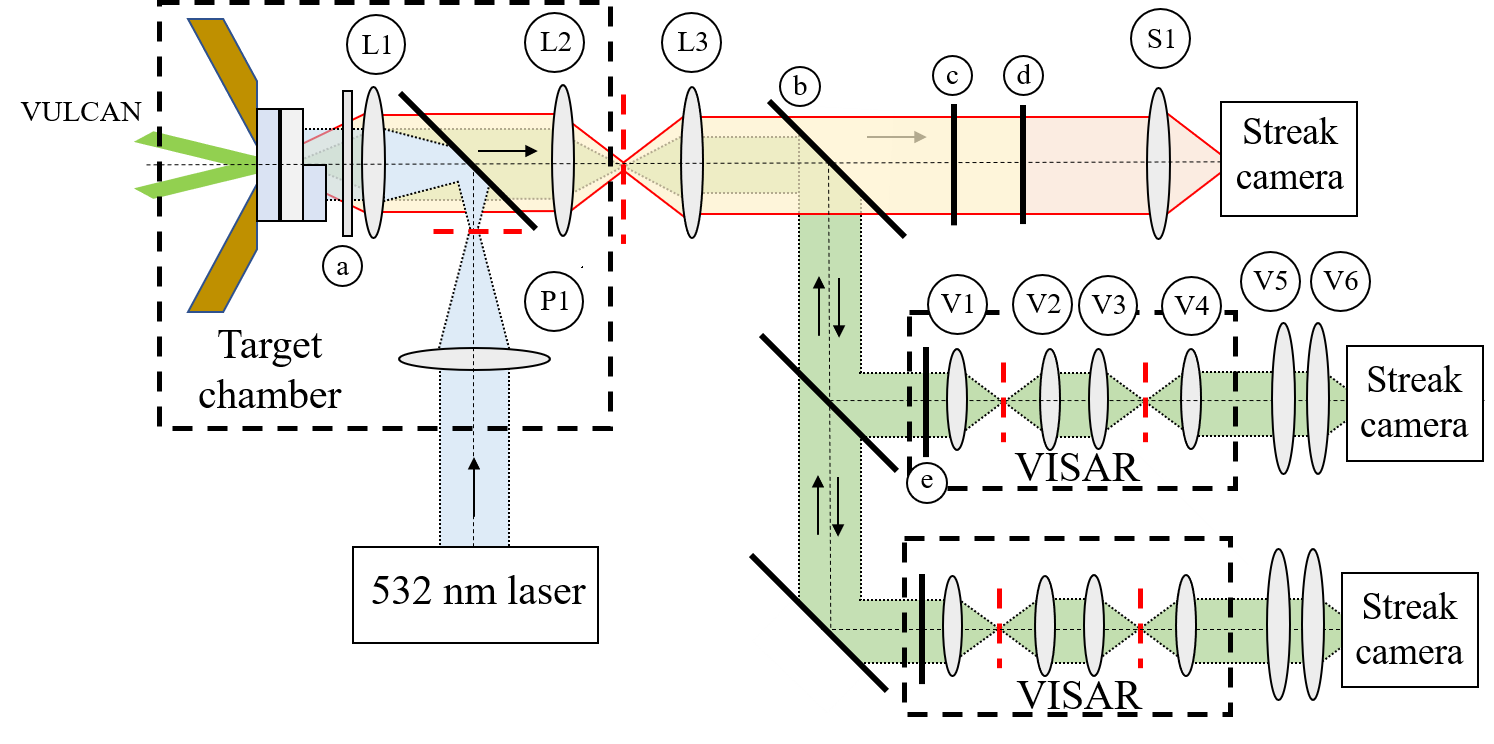
\includegraphics[width=0.8\textwidth]{figures/Experiment/SuggestedSchematic.png}% Here is how to import EPS art
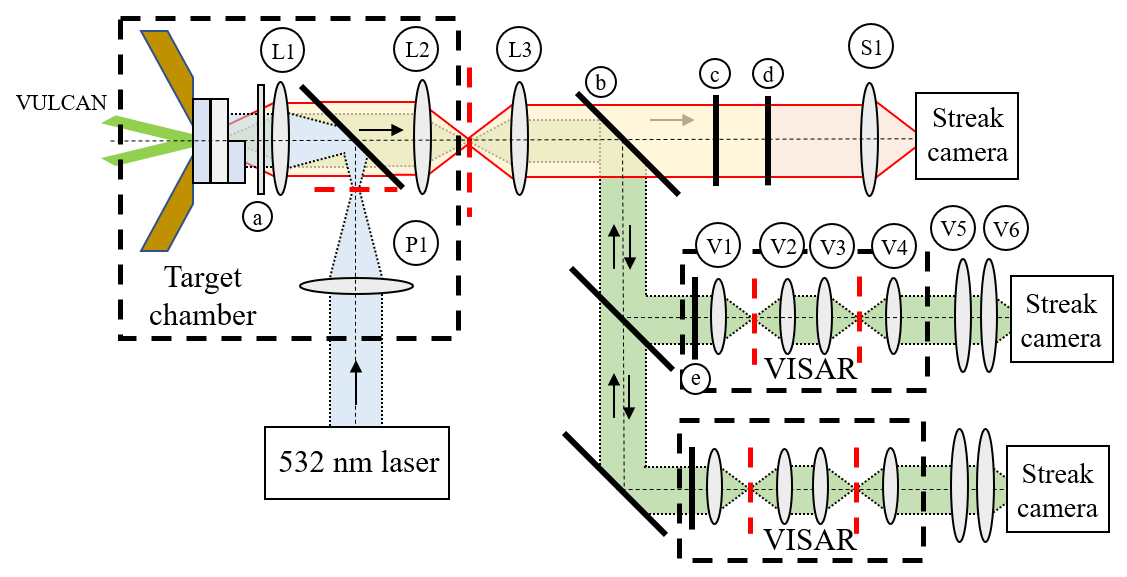
\includegraphics[width=0.8\textwidth]{figures/Experiment/SchematicsWithBackgrounds/ImprovedSchematic.png}% Here is how to import EPS art
\caption{\label{fig:SuggestedSchematic} Schematic of the suggested new setup. All labelled components are as for the previous setups, except the focal lengths of some lenses have changed: L2 is now 1000mm, L3 is 300mm, S1 is 400mm, and the first lens in each VISAR (V1) is now 500mm. This schematic does not have the beam collimated as it leaves the chamber, but it would be possible to include this if required.}
\end{centering}
\end{figure}

\begin{figure}
\begin{centering}
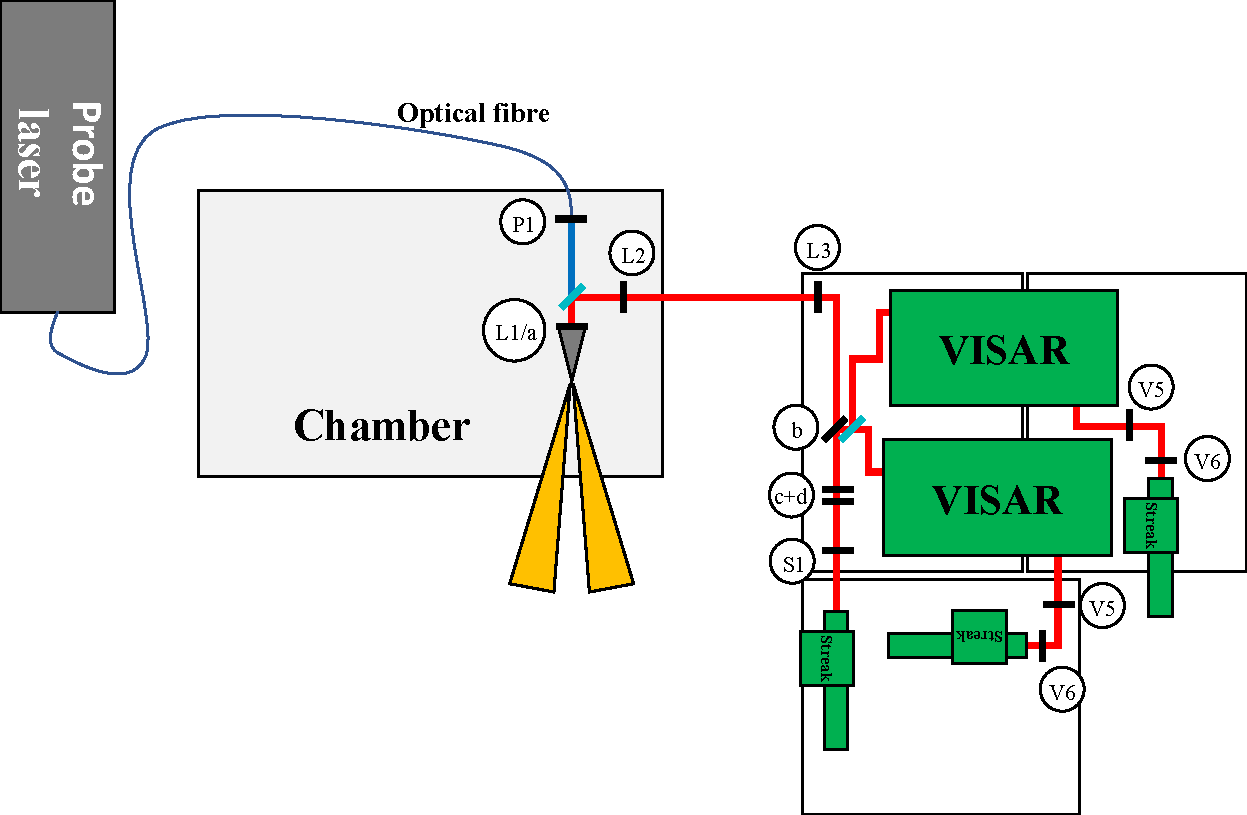
\includegraphics[width=0.8\textwidth]{figures/Experiment/ImprovedSetup.pdf}% Here is how to import EPS art
\caption{\label{fig:SuggestedSetup} A suggested spatial arrangement for the new setup displayed in Figure \ref{fig:SuggestedSchematic}, with labels as in the previous figures. This setup gives appropriate optical path lengths to minimise losses, while satisfying all other spatial requirements. No full CAD model of this setup has been produced; this is not accurate to scale, and the lengths in this image are thus approximate.}
\end{centering}
\end{figure}

\section{Conclusion}
The results of the experiment have been analysed. It was found that, for the 20 - 120 \unit{\giga\pascal} pressure range considered, the compression behaviour of the 260 \unit{\milli\gram\per\centi\meter\cubed} TMPTA foam was well described using QEOS and SESAME equation of state models for CH plastic. These equation of state models assume the foam to be a low-density homogenous plastic, and this agreement thus suggests this approximation can be used to obtain a reasonable description of the foam under these conditions. While the equation of state models overestimated the experimentally-measured shock temperatures, a lack of confidence in these measurements due to poor signal strength means that further data would be required to make firm conclusions on this topic.

It was observed in the data that the shock strength in the quartz was significantly lower than expected, based on both simulations and from shock-propagation times through previous layers of the multi-layer target. After assessing the evidence, it was suggested that a partial delamination of the quartz from the previous layers may be a likely explanation for this. Further comparison was made of the experimental results to simulations in a variety of 1D and 2D codes, and a range of potential improvements that could be implemented in a follow on experiment were suggested.